
%%%%%%%%%%%%%%%%%%%%%%%%%%%%%%%%%%%%%%%%%
% Arsclassica Article
% LaTeX Template
% Version 1.1 (10/6/14)
%
% This template has been downloaded from:
% http://www.LaTeXTemplates.com
%
% Original author:
% Lorenzo Pantieri (http://www.lorenzopantieri.net) with extensive modifications by:
% Vel (vel@latextemplates.com)
%
% License:
% CC BY-NC-SA 3.0 (http://creativecommons.org/licenses/by-nc-sa/3.0/)
%
%%%%%%%%%%%%%%%%%%%%%%%%%%%%%%%%%%%%%%%%%

%----------------------------------------------------------------------------------------
%	PACKAGES AND OTHER DOCUMENT CONFIGURATIONS
%----------------------------------------------------------------------------------------

\documentclass[
11pt, % Main document font size
a4paper, % Paper type, use 'letterpaper' for US Letter paper
oneside, % One page layout (no page indentation)
%twoside, % Two page layout (page indentation for binding and different headers)
headinclude,footinclude, % Extra spacing for the header and footer
BCOR5mm, % Binding correction
]{scrartcl}


\input{structure.tex} % Include the structure.tex file which specified the document structure and layout

\hyphenation{Fortran hy-phen-ation} % Specify custom hyphenation points in words with dashes where you would like hyphenation to occur, or alternatively, don't put any dashes in a word to stop hyphenation altogether
\fontfamily{roboto}


\lofoot{Thomas Moffat, 51337, 4042}
\lefoot{Thomas Moffat, 51337, 4042}

%----------------------------------------------------------------------------------------
%	TITLE AND AUTHOR(S)
%----------------------------------------------------------------------------------------


\setcounter{LTchunksize}{10}

%----------------------------------------------------------------------------------------

\begin{document}

%----------------------------------------------------------------------------------------
%	HEADERS
%----------------------------------------------------------------------------------------

\renewcommand{\sectionmark}[1]{\markright{\spacedlowsmallcaps{#1}}} % The header for all pages (oneside) or for even pages (twoside)
%\renewcommand{\subsectionmark}[1]{\markright{\thesubsection~#1}} % Uncomment when using the twoside option - this modifies the header on odd pages
\lehead{\mbox{\llap{\small\thepage\kern1em\color{halfgray} \vline}\color{halfgray}\hspace{0.5em}\rightmark\hfil}} % The header style

\pagestyle{scrheadings} % Enable the headers specified in this block

%----------------------------------------------------------------------------------------
%	TABLE OF CONTENTS & LISTS OF FIGURES AND TABLES
%----------------------------------------------------------------------------------------

\begin{titlepage}
	\vspace{5cm}
	\centering
	{\huge\bfseries ORDR: An Sports Club kit-ordering system\par}
	\vspace{2cm}
	{\Large\itshape Thomas Moffat\par}
	\vspace{1cm}
	{Candidate Number: 4042\par}
	\vspace{1cm}
	{Centre Number: 51337\par}
	\vspace{10cm}
	{Report generated using \LaTeX}
	\vfill
\end{titlepage}

\setcounter{tocdepth}{3} % Set the depth of the table of contents to show sections and subsections only

\tableofcontents % Print the table of contents

\listoffigures

\listoftables

%----------------------------------------------------------------------------------------
%	ABSTRACT
%----------------------------------------------------------------------------------------


%----------------------------------------------------------------------------------------
%	AUTHOR AFFILIATIONS
%----------------------------------------------------------------------------------------



%----------------------------------------------------------------------------------------

%\newpage % Start the article content on the second page, remove this if you have a longer abstract that goes onto the second page

%----------------------------------------------------------------------------------------
%	INTRODUCTION
%----------------------------------------------------------------------------------------

\section{Analysis}
\subsection{Background to and Identification of the Problem}
The client for this program is Kira, my mother, who volunteers as a kit orders organiser for Tilehurst Swimming Club, who asked me to develop a solution for her to be able to organise kit orders more effectively. \par The current system is paper-based, so it is very slow and very inconvenient for her as it requires her to spend vast amounts of time filling in a spreadsheet in order to organise an order, and then she has to copy it all out of the spreadsheet into an email to send off to the kit suppliers. A computerised solution would alleviate some of the time required to do this and might even allow her to automate most of it.

\subsection{Interview With Primary User}
\begin{itemize}
\item What is the current system?\par

The current system is manual and uses either a paper form with a BACS (Bankers Automated Clearing Service), cheque or cash payment or an email of the same form with usually a BACS payment (sometimes a cheque delivered later) with all the relevant data being entered onto a spreadsheet for record keeping.
The data is then transferred manually to an order sheet that is used to place the order at the printers. 

The initial data required to be processed and kept track of by the club is -  Name, Number, Garment Type, Size, Personalisation, Cost, Total Cost and Payment Made.

The data required for the order sheet that is given to the printers requires only Garment Type, Size and Personalisation and is categorised by Garment Type.

\item What are the benefits of the existing system?\par
At the time of set up, this system did not require a lot of time to implement.

\item What are the drawbacks?\par
Due to its simplicity, the current system is time-consuming. Each order requires a lot of manual entry and data processing, which could easily be achieved in a more automated way. Data can get lost in between the order spreadsheet and the order sheet that is sent to the printers.

\item Which new features would be most useful?\par
\begin{itemize}

	\item A usable interface to enter the order data by the parents or by the person with the responsibility for kit ordering in the club.
	\item Storage of this data in a usable way.
	\item Automatic creation of the order sheet from the initial data on a monthly basis
	\item Emailing the order sheet to the printer with a covering email.
	\item Ability to send an email to the parents to update them with the order status.
	\end{itemize}

\item Which existing features would you like kept?\par

The new system should be based on the old system but be a better version.

\item Who would be using this system?\par
\begin{itemize}
	\item On the front end?\par
	The swimmers or swimmers’ parents or the kit order person.
	\item On the back end?\par
	The kit order person.
\end{itemize}

\item How often would you expect to be using the system?\par

The system would be used monthly to create the order sheet for the printers.

\item How often would you expect others will use the system?\par

Parents or swimmers could use the system daily to place orders.

\item Will you need any security on it?\par

Security for email addresses.
\end{itemize}

\subsection{The Current System}
The current system is paper-based, so people wanting to order kit have to download a form from the club website then fill it in and either hand it in on one a Friday night or email it to the kit email address, which then requires Kira to collate all of these orders in to one before then sending it off to the manufacturers. The kit form is seen here:
\par 
\begin{figure}[h]
	\centering
	\includegraphics[scale=0.5]{TSCKitOrderForm}
	\caption{The current order form}
	\label{TSCOrderForm}
\end{figure}
\par This is obviously a very slow system, especially as the orders only get placed once a month, so it can take up to a month to receive kit that has been ordered, and possibly longer if the orders have been forgotten, which has happened far too many times in the past. This also has the problem of wasting a large amount of paper, as the forms are just collated on the computer and then discarded. \par 
Yet another problem with this system is that it requires everyone to pay attention to the dates, as missing the deadline could mean a wait of another month, and if the kit has been ordered for a large competition then it could very easily mean that the swimmers don't get what was ordered in time for the competition, as it normally takes a couple of weeks for all of the ordered kit to be printed and then picked up again. After the orders have been placed and then received, it requires Kira to email out to all the parents that their kit has been received and then requires her to bring it to a Friday-evening session when the parents are also present, and not all of the members of the squads, especially in the lowest squad swim on Fridays, so it can be a few weeks or months before the swimmers actually get the kit that was ordered. The objective for this project then, is to make a way for parents to order kit and then for Kira to be able to collate this together without hours of data entry.

\subsection{Prospective Users}
The prospective main users of this system will be Kira and then whomever takes over from her when she steps down as Kit Organiser. For this reason, I will need to assume that the users of this system are not tech-savvy, due to the fact that, while I know that Kira knows how to use computers fairly well, I don't know who will be following her so I don't know what their capabilities are regarding computers. For this reason the solution will have to be very simple so that people of any ability can use the system. \par 
The secondary users of this system will be the parents that are ordering kit using a form on the club website, so the forward-facing system will have to be very easy to use, as I don't know all of the parents so I have to assume that some of them will be tech-illiterate, or at the very least, uncomfortable with computers. 

\subsection{User Needs and Acceptable Limitations}
 Kira needs to have a way that she can have the parents order what they want and then have it in a searchable database so that she can just create an email to send to the kit manufacturers once a month. Then when she receives the kit she wants to be able to send out a mass email to the people who have ordered kit the previous month that tells them their kit is ready to be picked up. 
 \par Although the parents of the swimmers won't be the primary users, they will be affected quite a lot by the system, so it should be easy to navigate and similar in layout to the paper order form, to facilitate change-over. They will need a way to order kit, in an simple layout that then makes sure they know when their kit has been ordered and when it has come in.
 \par The acceptable limitations for this will be:\begin{itemize}
 	\item The hardware this will be running off will be somewhat underpowered, as if it is hosted locally it will be running off a 2009 MacBook Pro, and otherwise, if it is web-based it will be running on the club's web server which is not configured for a large volume of data and a large number of users using it at once.
 	\item My skills and knowledge - The system will have to not be too complex for me to create, as I have limited programming skills and limited resources. There are a few ways I could make this system, so I will have to be careful to not choose an overly simple solution, just because it is easy.
 	\item Time constraints - This system will need to be finished by February half term.
 	\item Features not able to be implemented due to complexity - Although this is an order system, it will have to work on a trust-based system as it would be far too complex for me to add in a payment solution, either involving BACS or something else. For this reason, the payments will still be processed manually, and people who haven't paid will be chased up in person. 
 	
 \end{itemize}

\subsection{Data Sources and Destinations}
The sources of data are the parents ordering kit, by way of the order form and Kira entering the details into an Excel spreadsheet. This source will not change with the new system, however it won't be via Kira, it will be automatically added in to a database. In the current system the spreadsheet is printed out and then sent off to the kit manufacturer and then Kira receives an email when they are ready for the kit to be picked up. In the new system, the data would again be arranged into a spreadsheet and printed out. This is an unfortunate limitation of the kit suppliers, not a problem on the club's end.
\begin{table}[ht]
	\small
	\caption{Current Data Sources and Destinations}
	\centering
	\makebox[\linewidth]{
	\begin{tabular}{|c|c|c|}
		\hline
		What is it & Source & Destination \\ [0.5ex]
		\hline
		Customer Details & Parents filling in an order & Excel Spreadsheet \\
		Order & Parents filling in an order & Spreadsheet \\
		Order Details & Excel Spreadsheet & Word Document\\
		\hline
		\end{tabular}}
\end{table}\par
\begin{table}[ht]
	\small
	\caption{Proposed Data Sources and Destinations}
	\centering
	\makebox[\linewidth]{
	\begin{tabular}{|c|c|c|}
		\hline
		What is it & Source & Destination \\
		\hline
		Customer Details & Parents filling in an order & customerDatabase \\
		Order details & Parents ordering kit & orderDatabase\\
		Admin Details & Kit Organiser & orderDatabase\\
		Order Details & orderDatabase & Word Document or Email\\
		\hline
		\end{tabular}}
\end{table}

\subsection{Data Volumes and Data Dictionaries}
The volume of data will be very low as the system will work entirely in text, only one person will be accessing the back-end of it, the volume of kit orders is fairly low, although high enough for this to be a problem. Also, this will only be accessed once or twice a month so the data volumes will be kept low. \par A rough calculation (using the data in Table 4) would suggest that, per order, 1156.25 bytes will be produced (i.e. 1156 bytes, 2 bits). This would suggest that, at an average order size of about 10 orders per month, the system will produce about 10kB of data per month. This is an average, there will be more produced in the run up to the large competitions of the year, and less after said competitions. 
\begin{table}[ht]
	\small
	\caption{Current Data Dictionary}
	\centering
	\makebox[\linewidth]{
	\begin{tabular}{|c|c|c|}
		\hline
		Data & Data Type & Description\\
		\hline
		Name & Text & Name of the customer\\
		Order & Text & What the customer ordered\\
		Order Quantity & Number & How many of each item was ordered\\
		Paid & Text & Shows how the customer has paid\\
		Email address & text & Customer's email address\\
		Squad & text & What swimming squad the child is in\\
		Name on back & text & what name the customer would like printed\\
		Size & text & what size the clothes are\\
		Cost & text/numbers & how much the overall cost will be\\
		\hline
		\end{tabular}}
\end{table}
\begin{table}[ht]
	\small
	\centering
	\caption{Proposed Data Dictionary}
	\makebox[\linewidth]{
	\begin{tabular}{|c|c|c|c|c|c|}
		\hline
		Field Name & Purpose & Type & Typical length (B) & Example & Validation \\ [0.5ex] % inserts table %heading
		\hline
		Name & Stores name of customer & String & 40 (320) & Alex & Not blank \\
		Ordered Kit & Stores type of kit ordered & String & 40 (320) & Polo shirt & Not blank \\
		Quantity ordered & stores number of each item & Integer & 2 (4) & 1 & >-1, <100 \\
		Paid? & Stores if order has been paid & boolean & 1 (1/8) & True & true or false \\
		Ordered & stores if order has been placed & bool & 1 (1/8) & True & true or false \\
		Email address & stores email address & String & 47 (376) & abc@abc.com & Not blank\\ 
		Name on back & stores name printed on the back & String & 10 (80) & Pedro & Not blank\\
		Squad & stores what squad swimmer is in & String & 3 (24)& Top & Not blank\\
		Size & size the items of clothing will be & String & 4 (32)& M & Not blank\\[1ex]
		\hline
		
	\end{tabular}}
	
\label{table:nonlin}
\end{table}


\subsection{Data Flow Diagrams}
\begin{figure}[H]
	\centering
	\includegraphics[width=\textwidth]{CurrentLvl0}
	\caption{A level 0 data flow diagram of the current system}
	\label{CurrentLvl0}
\end{figure}
\begin{figure}[H]
	\centering
	\includegraphics[scale = 0.35]{CurrentLvl1}
	\caption{A level 1 data flow diagram of the current system}
	\label{CurrentLvl1}
\end{figure}
\begin{figure}[H]
	\centering
	\includegraphics[width=\textwidth]{ProposedLvl0}
	\caption{A level 0 data flow diagram of the proposed system}
	\label{ProposedLvl0}
\end{figure}
\begin{figure}[H]
	\centering
	\includegraphics[width=\textwidth]{ProposedLvl1}
	\caption{A level 1 data flow diagram of the proposed system}
	\label{ProposedLvl1}
\end{figure}
The proposed system as seen in figure \ref{ProposedLvl1} is rather more complicated than the current system seen in figure \ref{CurrentLvl1} which unfortunately means that there are more things that will need to be kept track of and so more things that could potentially break, however this will be traded off with a massive increase in convenience for everyone, not to mention that most of the system can be automated which will reduce the kit coordinator's workload. This will also mean that the system will be much faster, as orders will be entered into the system immediately and so will not be forgotten, unlike in the current system.

\subsection{Entity Relationship Models}
The current entity relationship model can be seen in Figure \ref{CurEER}, and this is a rather abstract view of what requires a lot of paper and back and forth.
\begin{figure}[H]
	\centering\includegraphics[width=\textwidth]{ERCurrentDiagram}
	\caption{The current Entity Relationship Diagram}
	\label{CurEER}	
\end{figure}

\begin{figure}[H]
	\centering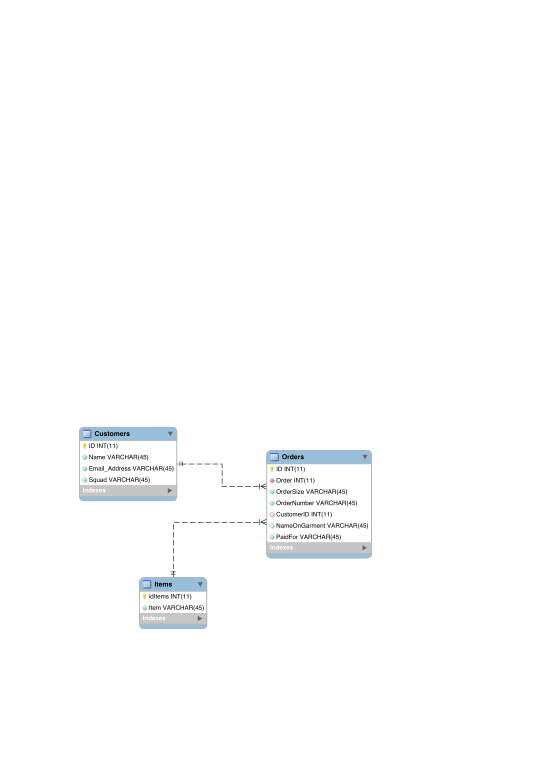
\includegraphics[width=\textwidth]{EERProp}
	\caption{The proposed Entity Relationship diagram, exported from MySQLWorkbench}
	\label{PropEER}	
\end{figure}
As can be seen in figure \ref{PropEER}, the proposed EER will be fairly simple, with some foreign keys.

\subsection{Entity Description}

Customer(\uline{ID}, Name, Email\_Address, Squad)\\
Order(\uline{ID}, Order (Foreign key from Items), OrderSize, OrderNumber, CustomerID (Foreign key from Customer), NameOnGarment)\\
Items(\uline{idItems}, Item)

\subsection{Objectives for the Proposed System}
The objectives of this system are to have an easy to use system that will run on minimal hardware. More specifically  \begin{enumerate}
	\item It must have a well-structured (1NF or 2NF) database system that can be easily accessed.
	\item It must have some sort of user interface allowing a person to enter the data then have the program handle the sorting.
	\item It must store the data in a usable way (Most likely plain text).
	\item It must have a search function, so the kit coordinator can search the database for certain attributes, like, for example, people who have and haven't paid for their order.
	\item It must be lightweight enough to be run on a web server, such as the one hosting the club website.
	\item It should have a way to automate the kit ordering procedure, by generating the order form that is sent off to the kit printers.
	\item It should have a web-based front end so the orders for kit can be placed via the club website.
	\item It could be able to send a mass email to all of the people who have ordered kit.
	\item It could have an ability to monitor the email inbox of the kit email address so when the printer emails that the kit is ready it will send out a mass email automatically to everyone that has ordered.
	\item It would be nice to have an integrated payments solution so everything could be done through the web interface, although due to time and complexity constraints this probably won't happen.
\end{enumerate}

\subsection{Potential Solutions}
The potential solutions for this project are:\begin{itemize}
	\item An Excel spreadsheet using a VBA front-end application
	\item A VB.NET front-end application and a Microsoft Access database on the back-end
	\item A fully bespoke system programmed in Java and HTML
	\item A fully bespoke system programmed in C++
\end{itemize}
The respective advantages and disadvantages are seen in the next section.

\subsection{Feasibility of Potential Solutions}
\begin{itemize}
	\item An Excel spreadsheet using a VBA front-end. Advantages:\begin{itemize}
		\item It would be exceedingly easy to implement, as it just requires a spreadsheet and a small amount of programming to get up and running.
		\item User already has experience using Excel and so would be able to use the system with minimal help.
	\end{itemize}
	Disadvantages:\begin{itemize}
		\item This solution would be offline only, so one of the main features of the proposed solutions, the online ordering system, would have to be left out, or radically changed.
		\item Excel is a flat file database, which doesn't lead to good database design practices and also won't let me handle links between data.
		\item The current system involves Excel so the new system would be too similar to the current system, and so wouldn't follow what the client wanted. 
	\end{itemize}
	\item A VB.NET front-end application and a Microsoft Access database back-end. Advantages:\begin{itemize}
		\item Most of the system is pre-implemented so it would require a minimal amount of work to get up and running.
		\item Unlike the Excel spreadsheet, data can be linked to and the database won't be just flat.
	\end{itemize}
	Disadvantages:\begin{itemize}
		\item I have no experience using VB.NET, which would add an unnecessary level of complexity to the project, as I would need to learn VB.NET as I worked.
		\item I don't have convenient access to a copy of Microsoft Access, which would mean that I would need to purchase a copy.
		\item The solution will be offline only, which will mean that orders wouldn't be able to be placed through the website.
		\end{itemize}
	\item A bespoke coded system in Java. Advantages:\begin{itemize}
		\item It would allow me to control and integrate everything from the beginning, as I would be creating most of the system from scratch.
		\item There would be no outlay, as I can use a free IDE to develop in, and Java which is itself free.
		\item The system won't be a flat file database, so I will be able to have links between data.
		\item Thanks to JDBC, the database will be searchable using SQL statements.
		\item The solution will be able to be hosted online and allow the kit coordinator to log in to the back end to view the database.
	\end{itemize}
	Disadvantages:\begin{itemize}
		\item Java can be unnecessarily complex to write a program in.
		\item Java can be a massive resource hog, which means that it would be tricky to run on a low-budget web server.
		\item I have minimal experience programming in HTML.
	\end{itemize}
	\item A bespoke coded solution in C++. Advantages:\begin{itemize}
		\item C++ is a fairly low-level language, so it's quite powerful
		\item It has a large community, so if I get stuck with a problem then I can research solutions with little time wasted.
	\end{itemize}
	Disadvantages:\begin{itemize}
		\item I have absolutely no knowledge of programming using C++ so I would have to spend a lot of time learning how to code using it, which could be better spent programming the solution. 
		\item Is apparently not very good for cross-platform applications, as a library is normally chosen which is platform specific, although due to my lack of knowledge of this language I don't know if this is true or not.
	\end{itemize}
\end{itemize}

\subsection{Justification of Chosen Solution}
I will be making a bespoke solution in Java for this project, as I have far more experience in this language than any of the other solutions that I proposed. I also feel this will be the best as Java is incredibly versatile, and so can be run on any platform with minimal amounts of set-up. It does not require any purchase to be made, unlike Microsoft products which means that it can be made on a shoestring budget. \par Also due to Java's ubiquity it has a vast number of resources that will be very helpful for referring to, if I get stuck with a certain section of this project. It has very good integration with SQL thanks to JDBC, which will mean that everything can be integrated into one complete package, rather than relying on solutions that could break if there is an update to the commercial software package being used. This integration will also mean that I will be able to make the database searchable via SQL queries, which will definitely improve workflow as the kit organiser will be able to search for, for instance, people who haven't paid. \par Although Java is normally seen as quite a resource intensive language, I think that, if the program stays small it will be relatively lightweight to run on the server. I will be able to deal with the relative complexity of Java as a language by ensuring that my design is logical and methodical. \par While I do have minimal experience using HTML, I feel that this will be the easiest way to create a web form, as opposed to coding an applet in Java. This is due to the fact that I experimented with making a JApplet and decided that it was too convoluted for what I wanted to do and would have bogged me down, trying to get it to work. 




\section{Design}

\subsection{Overall System Design}
\begin{table}[H]
\small
\centering
\caption{Summary Table}
\makebox[\linewidth]{
\begin{tabular}{|c|c|}
	\hline
	Inputs & Processes \\ [0.5ex]
	\hline
	Swimmer's name & Add new Order\\
	Email Address & Add new customer\\
	Squad & Compile order to send off\\
	Name on Garments & Edit order\\
	Order & Show all orders to Kit Co-ordinator\\
	Size of the Garment & \\
	Number of Garments ordered & \\
	Whether the order has been paid for & \\
	\hline
	Tables Storing Data & Outputs\\ [0.5ex]
	\hline
	Order Details & Compiled Order Form \\
	Customer Details & Certain Orders via Search Function \\
	Items Available & All orders in table to kit co-ordinator\\
	\hline
	
	
\end{tabular}}
\end{table}

\subsection{Description of Modular System Structure}
Figure \ref{Customer} shows the process when the web page with the order form is filled out and submitted. This allows the program to remain streamlined in that the user just has to click submit and everything is hidden from them and put into the database automatically. This then makes it easier on the Kit Coordinator as they don't have to deal with any more paper, they can use the rest of the program to access the database and perform administrative tasks on it such as generating the contents of the database into a spreadsheet (more on that later)
\begin{figure}[H]
\centering
\includegraphics[scale=0.5]{customer}
\caption{The part of the project facing the customer. This is all written in web-based technology}
\label{Customer}
\end{figure}
\begin{figure}[H]
\centering
\includegraphics[scale=0.5]{KitCoordinator}
\caption{The part of the project facing the Kit Coordinator. This is all written in Java, except for the SQL script and the CSV}
\label{KitCoordinator}	
\end{figure}
Due to the relative complexity of the Java end of the project, the functions are given in a slightly more easy to follow format in tables 6 and 7, which shows the main functions as you drill down into the program. This is marginally easier to follow than figure \ref{KitCoordinator} due to the fact it follows a slightly more logical layout, although figure \ref{KitCoordinator} gives a more complete view of what is going on in the program as a whole. These diagrams are most useful when used together for the design as figure \ref{KitCoordinator} gives a better view of the inputs and outputs of the programs while tables 6 and 7 show the structure of the program better. \par The main feature here is the function to generate an order form that outputs as a spreadsheet, as this allows the Kit Coordinator to click a button and have a correctly formatted order form to be generated and then sent off to the printers. This saves time and effort, as the Kit Coordinator doesn't have to spend large amounts of time transcribing the order forms by hand into an Excel spreadsheet and then sending that off to the printers. Instead the spreadsheet can be generated. The reset function can be useful if something goes horribly wrong with the database, such as someone gains access to it and defaces it, the Kit Coordinator can just click a button and the database is remade completely fresh and blank.
\begin{table}[H]
\tiny
\centering
\makebox[\linewidth]{
\begin{tabular}{|c|c|c|c|c|c|c|c|c|c|}
\hline
Ordr &  &  &  &  &  &  &  &  &  \\ 
\hline
MainMenu &  &  & Get Connection &  &  & Remake Database &  &  & \\ 
\hline
Display & Enter Sort & Enter Search String & Open XML File & Get Connection Details & Return & Open SQL File & Run Script & Open CSV & Execute\\ 
\hline 
\end{tabular}}
\label{table:tdd1}
\caption{\small{Part 1 of top down design}} 
\end{table}
\begin{table}[H]
\tiny
\centering
\makebox[\linewidth]{
\begin{tabular}{|c|c|c|c|c|c|c|}
\hline
Ordr & & & & & & \\
\hline
Show Contents with search &  &  &  & Show Contents &  & \\ 
\hline
Get Search & Get Ordering & Execute SQL Query & Show Contents & Get Ordering & Execute SQL Query & Show Contents\\ 
\hline
\end{tabular}}
\label{table:tdd2}
\caption{\small{Part 2 of top down design}}
\end{table}





\subsection{Design Data Dictionary}
For the purposes of this, B is the length of the field in bits. This is all assuming that the text is encoded in UTF-8, which allows for internationalisation. The only validation method given for most of these is that they aren't null. They're just required to be present. This is because the validation will be performed using HTML forms, and the data types that it allows. So the email address box on the form will have an email type, etc. The items of kit for the order form will be in a drop-down menu so there isn't really any way that they can be altered, at least not in normal use. This is similarly true of the Squad and the Payment Method. The number of garments will be chosen with an upper limit of one and a lower limit of five, so there's no real way to have strange values, such as -1. The PaidFor option is just a radio on the webpage, so there shouldn't be any strange values. In this case MySQL won't accept the value anyway if it isn't 0 or 1, as it is a boolean. 
\begin{table}[ht]
	\small
	\centering
	\caption{Customer Table Data Dictionary}
	\makebox[\linewidth]{
	\begin{tabular}{|c|c|c|c|c|c|}
		\hline
		Field Name & Purpose & Type & Typical length (B) & Example & Validation \\ [0.5ex] % inserts table %heading
		\hline
		ID & Differentiate Customer & Int & 3 digits max (16) & 2 & It's generated by MySQL \\
		Name & Stores Customer Name & String & 40 (640) & Joe Bloggs & Not null \\
		Email & Stores Email address & String & 40 (640) & abc@abc.com & Not null, is an email address \\
		Squad & Stores Swimmer's squad & String & 3 (48) & Top & Not null \\[1 ex]
		\hline
		\end{tabular}}
	\label{table:cusdatdic}
\end{table}
\par Table \ref{table:cusdatdic} shows the columns in the Customer table of the database, with all the datatypes etc. All the strings in this table are set to VARCHAR(45), i.e. if the strings are longer than 45 characters, they aren't accepted by the database and the query isn't updated. This length was chosen as it will be very unlikely to find a name or email address longer than that length in every day testing, and if a fringe case like that does come up then the database can be altered to allow longer email addresses to be used. As  an example, Chargoggagoggmanchauggagoggchaubunagungamaugg is 45 characters, which is a very long place name and there will be almost no email addresses longer than this, unless said email address was chosen as a joke. This is why the typical length is set to 40 in the case of both the Name and the Email Address column, as this length is considered to be a fringe case so that data usage can be calculated as if every single name and email address was that length and a worse case scenario can be found.
\begin{table}[ht]
	\small
	\centering
	\caption{Order Data Dictionary}
	\makebox[\linewidth]{
	\begin{tabular}{|c|c|c|c|c|c|}
		\hline
		Field Name & Purpose & Type & Typical length (B) & Example & Validation \\ [0.5ex] % inserts table %heading
		\hline
		ID & Stores the Order ID & Int & 3 digits max (16) & 3 & Auto-generated by MySQL \\
		Orders & Stores the Item ID & Int & 1 (16) & 4 & Retrieved from Items \\
		OrderSize & Shows the size of the item & String & 5 characters max (80) & M & Not null \\
		OrderNumber & Number of the item ordered & Int & 1 (16) & 1 & Not null \\
		CustomerID & Stores the ID of the customer & Int & 3 digits max (16) & 4 & Retrieved from Customers \\
		NameOnGarment & Stores string put on item & String & 5 (80) & Pedro & Not null \\
		PaidFor & Whether item has been paid for & Bool & 1 (1) & 0 & Not null \\
		PaymentMethod & Stores payment method & String & 4 (64) & BACS & Not null \\[1ex]
		\hline
		
	\end{tabular}}
	\label{table:orddatdic}
\end{table}
\par Table \ref{table:orddatdic} shows the columns within the Orders table of the database. While the strings are all set to VARCHAR(45) again, most of the fields will be changed using drop down boxes, so the length of the field is overkill. This is to facilitate easy changing in the future if the length of some option suddenly became far longer. The only string in this table that isn't chosen from a drop-down menu is the NameOnGarment column, which has a 'social limit' in that most people have nicknames on the backs of their T-Shirts or Hoodies that don't extend to any more than 8 characters, and normally fewer, and people have their initials on their bags, which is normally four or fewer characters. So the VARCHAR(45) field here is still overkill, however it is still there if the customer wants the option to have a fabulously long name on the back of their T-Shirt (the bags don't have enough room to have anything other than initials printed on them).
\begin{table}[ht]
	\small
	\centering
	\caption{Items Data Dictionary}
	\makebox[\linewidth]{
	\begin{tabular}{|c|c|c|c|c|c|}
		\hline
		Field Name & Purpose & Type & Typical length (B) & Example & Validation \\ [0.5ex] % inserts table %heading
		\hline
		idItems & Stores item ID & int & 1 (16) & 5 & Auto-generated by MySQL \\
		Items & Stores item name & String & 7 (112) & Polo Shirt & Input on initialisation \\[1 ex]
		\hline
		
	\end{tabular}}	
\label{table:itedatdic}
\end{table}
\par Table \ref{itedatdic} shows the two columns from the Items table in the database. This is never directly altered except for when the remake button on the program is clicked, and the program accesses a CSV file with the values to be inserted into the table, and then populates this table. This table could be set to read-only to prevent vandalism or mistakes, however this could raise problems further down the road so will not be implemented during the initial stages of this program.
\begin{table}[H]
	\small
	\centering
	\caption{Connection XML Data Dictionary}
	\makebox[\linewidth]{
	\begin{tabular}{|c|c|c|c|c|c|}
		\hline
		Field Name & Purpose & Type & Typical length (B) & Example & Validation \\ [0.5ex] % inserts table %heading
		\hline
		dbms & Show database manager & String & 5 (80) & mysql & Not null \\
		database\_name & shows database name & String & 4 (64) & mydb & Not null \\
		user\_name & stores the user name & String & 5 (80) & root & Not null \\
		password & stores password & String & 8 (128) & cheetah & Not null \\
		port\_number & stores the port number & int & 4 (64) & 3306 & Not null \\
		server\_name & stores the server IP & String & 15 (240) & localhost & Not null\\[1 ex]
		\hline
		
	\end{tabular}}	
\label{table:conndatdic}
\end{table}
\par The last table, table \ref{table:conndatdic} is each of the nodes in the XML files kitorder.xml and kitorder2.xml. These are, I feel, self-explanatory, in that they do exactly what the node names say. They are retrieved when they are needed by a program. Note that there are two files that read exactly the same thing. The idea is that one will be kept locally with the java program (kitorder.xml) and the other (kitorder2.xml) will be loaded onto the web server, so they bother know how to find the database at all times. This came about during testing of the XML parsers in Java and PHP, and the XML parser in Java required the elements to be declared, while the XML parser in PHP kicked out an error when this was altered. This is very useful however as it allows the connection settings to be altered independently. 
\subsection{Database Design}
\begin{figure}[H]
	\centering
	\includegraphics[width=\linewidth]{KitOrderEERDesign}
	\caption{The EER for the designed system}
	\label{EERDesign}	
\end{figure}
Figure \ref{EERDesign} is the database diagram for the system as it is designed, this essentially takes the place of the order form in the original EER diagram seen in Figure \ref{CurEER}, except it requires far less paper to be wasted during the order process.
\subsection{Identification of Storage Material and Format}
The Java portion of this program will be stored on the user's computer, for them to connect to the database, which will be stored on the server that the swimming club's website is hosted on, in order to make the web form passing far easier, as this will obviously be hosted on the club's website as well, so just requires a localhost as opposed to a static IP or DNS lookup, which, while feasible, would be far harder to implement than having the website and server in the same place. This will be needed for the Java portion of the program, however this is going to be used far less often than the order form will, so it saves more time having the MySQL database on the website server. \par Most of the data will be written into and read from the database using SQL queries, as this is the only real way to input data into a table. When the database initialises, it will read in a SQL script and execute that using Mybatis, so a FileInputStream within Java; when the data from the database is output to an Excel spreadsheet then it will use a FileOutputStream within Java; and the connection settings, both in the Java end and the web end will use an XML parser from a FileInputStream on the Java end and a simplexml\_load\_file in PHP.\par The finished project will end up less than 100 MB, and most likely closer to 60, which would be including the Excel file as an output and all of the required libraries for the compiled .jar file. The raw source code will probably be less than 1MB.\par The backup system for the program will involve backing up the project when the website is backed up. The program itself will have a copy on the user's computer, then also on my computer and so in any backups I make using Backblaze, as well as a copy on Dropbox, and then the source code will be available on GitHub, so if everything goes wrong it will be feasible to retrieve the code and recompile it. If all three of GitHub, Dropbox and Backblaze go down then there's probably problems that are slightly more important than obtaining a copy of source code, but even then it will be stored on a physical USB stick kept with my computer.
\subsection{Identification of Processes and Algorithms for Data Transformation}
In this there will be a database search function, however this project will be using the ORDER BY function within MySQL as opposed to an algorithm due to how the data is handled when it is retrieved from the database, as it is retrieved as a ResultSet, and then converted into a map before being inserted into the TableView. So a bubble sort or shuttle sort would be unable to run on the data. The relevant section of code can be seen on lines 96-109 of Appendix A.3, or lines 105-118 of Appendix A.5. This is feasible as the volumes of data will be too small to justify a Bubble or Shuttle sort on the data and the MySQL ORDER BY will be fast enough for what is needed for this project. The SQL statements that will be used in this project are given here: 
\begin{lstlisting}[language=SQL]
	select o.ID, o.CustomerID, c.Name, c.Email_Address, c.Squad, o.Orders, o.OrderSize, o.OrderNumber, o.NameOnGarment, o.PaidFor, o.PaymentMethod, i.Item from Orders o INNER JOIN Customers c ON o.CustomerID = c.ID INNER JOIN Items i ON i.idItems=o.Order where o.ID like ? or o.CustomerID like ? or c.Name like ? or c.Email_Address like ? or c.Squad like ? or o.Orders like ? or o.OrderSize like ? or o.OrderNumber like ? or  o.NameOnGarment like ? or o.PaymentMethod like ? or i.Item  like ? ORDER BY;	
\end{lstlisting}
This first SQL query is the search query. This selects everything in the database where one of the columns matches the search query. The question marks are from the prepared statement in Java, and there would normally be a variable after the ORDER BY however this was cut off for readability in this report. This is the longest and most complex single SQL query in the whole project.
\begin{lstlisting}[language=SQL]
	select o.ID, o.CustomerID, c.Name, c.Email_Address, c.Squad, o.Orders, o.OrderSize, o.OrderNumber, o.NameOnGarment, o.PaidFor, o.PaymentMethod, i.Item from Orders o INNER JOIN Customers c ON o.CustomerID = c.ID INNER JOIN Items i ON i.idItems=o.Orders ORDER BY;
\end{lstlisting}
This SQL query is very similar to the previous one, the difference being that it doesn't have to be a prepared statement as the only user input is from a dropdown box, so the statement doesn't have to be protected in any way, due to the lack of attack vectors. Once again there would be a variable after the ORDER BY but this was cut out to improve readability.
\begin{lstlisting}[language=SQL]
	SELECT * FROM Customers INTO OUTFILE /Users/tsmoffat/kitordersystem/kitordersystem/kitordersystem/Customers.csv FIELDS ENCLOSED BY '"' TERMINATED BY ';' ESCAPED BY '"' LINES TERMINATED BY '\r\n'; SELECT * FROM Orders INTO OUTFILE /Users/tsmoffat/kitordersystem/kitordersystem/kitordersystem/Orders.csv FIELDS ENCLOSED BY '"' TERMINATED BY ';' ESCAPED BY '"' LINES TERMINATED BY '\r\n';
\end{lstlisting}
This SQL script is run to dump the contents of the Orders and Customers tables to CSV files so that they could be loaded back in to the database if need be. This script is run just before the database gets recreated by Mybatis in DBReset.jave, which can be found in Appendix A.7.
\par The last SQL query is actually a SQL script, and can be seen in full in Appendix A.8. This is the SQL script that is called when the entire database is rebuilt from the ground up. This is actually the most complex bit of SQL code, although it can't be called a query, as it is in fact a series of them, although Java does execute them all in the same update. 
 
\subsection{User Interface Design and Rationale}
The user interface will be constructed in JavaFX, as this is both easier to work with and better looking than swing. It also allows me to do some preliminary design work on the GUI in the program Scenebuilder, although, thanks to some more preliminary testing, this won't end up being the way I make this GUI. 
\begin{figure}
	\centering
	\includegraphics[scale=0.5]{UIDesign}
	\caption{The design for the Main Menu}
	\label{mmdes}	
\end{figure}
Figure \ref{mmdes} shows the design for the Main Menu of the Java end of the program. This is a very simple UI and so it is easy to understand, even if the user is unfamiliar with computers. This is the only screen with any real input. There is a text box once one clicks on the Remake button, but that is very linear, in that there are only two choice: input the phrase and click ok or close the box. This can be seen in figure \ref{confdes}.
\begin{figure}
	\centering
	\includegraphics[scale=0.5]{ConfirmBoxDesign}
	\caption{The design for the confirm text box. This will just use a JavaFX dialog box}
	\label{confdes}
\end{figure}
The final screen will show the contents and the results of the search query. As shown in Section 2.6, this will vary depending on the ordering and the search query in the case of the search display. 
\begin{figure}
	\centering
	\includegraphics[scale=0.3]{ContentsAndSearchDesign}
	\caption{The display of the contents and the search display. These will be generated dynamically}
	\label{searchdes}
\end{figure}
\par This UI is designed solely for people who have little experience using SQL. If they have prior experience using this then they either use this GUI if they want or they can bypass the GUI entirely and connect to the database using a terminal/command prompt and enter the commands directly, although this will mean that they won't be able to use some of the features of the program, such as the dump the relevant contents of the database to an Excel spreadsheet to be sent off to the manufacturers. Most of the functions to add a user or an order will be done by the users themselves on the webpage. The designs for these are shown by figure \ref{webcusdes}. These are quite simple to follow, with large buttons and text boxes to make it obvious what goes where. This facilitates ease of use for the customers,as some of them may not be particularly used to using computers.
\begin{figure}[H]
	\centering
	\includegraphics[scale=0.3]{CustomerDetailsInput}
	\includegraphics[scale=0.3]{OrderDetailsInput}
	\caption{The input forms on the internet}
	\label{webcusdes}	
\end{figure}



\subsection{Planned Data Capture and Entry}
	The planned data entry forms can be seen in Figure \ref{webcusdes}. The design was chosen to be easy to read, in nice large fonts with a good contrast. This is useful as a variety of ages will be using this web page and the aim is for it to be easy for everyone to read and to use. This is achieved through the minimal use of attention grabbing features, really the only one is the large, green submit button. It is also very easy to tell what goes where, either due to the large font on the drop-down menu or the label just above it which is easy to read. The text boxes are large, so that they can be selected easily, and to show that the length of string available is very long. In this case, the string that the customer can input is  limited to 45 characters although as discussed earlier the customer is unlikely to reach this limit as this length would accept a name as long as the third longest place-name in the world, which, suffice to say, is unlikely during normal usage. If a user runs into problems with the length of their name then this can always be increased. 
\subsection{Planned Valid Output Designs}
	The major output of this program is an Excel spreadsheet with all the relevant values from the table in it. Each item will be split into its own sheet, with the name of the customer, the size they want and what they want to be printed on the item input in columns on the respective sheet. This also includes hats and shorts as, even though the options for printing names on the hats and shorts isn't available at this moment in time, this allows for easy expansion in the near future. This output is slightly changed from the Analysis as, from some preliminary testing, the Java libraries that allow access to Word and Excel documents work half the time and then the other half, even with unchanged code, they don't. This level of reliability was unacceptable so the method chosen after this preliminary testing was to write a Python script that handles the output to the spreadsheet and then using Java to call and execute the Python script. This has proven to have a 100\% success rate and so will be the method that will be used in the final code.\par This program also outputs two CSV files when the remake function is called, which dumps the contents of the database so that it can be repopulated so no orders are lost if the database needs to be recreated for some reason. This is just a backup backup function, just in case the backups taken of the database can't be reloaded.
\subsection{Measures Planned for Security and Integrity of Data}
Most of the validation techniques are performed by MySQL, checking whether the values are null or whether they're over the character limit, etc. The email and the number of items are defined in the HTML source, the email as an email datatype and the number of items has a range defined between 1 and 5 so if the input string isn't an email address or the number of items is over 5 then the web browser will kick out an error and make them change it. SQL Injections are prevented by the use of Prepared Statements, which reduces this attack vector considerably. This means that there is no way that people should be able to gain a threshold into the database using this method. \par Error messages will be output in a dialog box with the error message and the stack trace for if the user is slightly more experienced with computers, or for troubleshooting purposes. These dialog boxes are the ones built in to JavaFX, with an expanded text box built in for displaying the stack trace. An example of this is available in Appendix C.2.2, Figure \ref{javaerrupdate}. \par If data input is incorrect then it goes into the database and requires a human to check it and alter it when it is output into an Excel spreadsheet, or the customer can submit a request to the Kit Coordinator to alter the record directly in the database, if the Kit Coordinator has the knowledge to do so. If not then the data will have to be modified manually in the Excel spreadsheet. The customer could also submit another form with the updated details and this will be taken as the more recent one and so used when the order sheet is being used, as long as there are no orders tied to that customer. If the order is messed up then they can submit another order and ask for the incorrect order to be taken off the order sheet. \par The backup solution has already been detailed, however it will be covered in more detail here. For this program, it will follow the 3-2-1 backup system, i.e. At least three backups, on at least two different storage mediums with at least one stored off site. In this case, the program source code is stored on my computer, on a flash drive and on GitHub. When the program goes into production, a backup will be taken of the database when the website itself is backed up. This will be stored with the web host, and a task will be set-up where the most recent back-up is downloaded whenever the database is backed up, then synchronised onto a NAS using an incremental backup job. This is to ensure that even if one or more of these systems goes down there is always a copy of the source code available. 

\subsection{Measures Planned for System Security}
The database will be password protected, and this will be administered through MySQLWorkbench, as this allows for multiple accounts to be created with different permissions. So when the program goes into production a user account just for the web end will be created that allows one to insert records and read them but do nothing else. This will help prevent vandalising the database, as the vandals will have no useful access. In production this connection will be protected by SSL, with a certificate signed by Let'sEncrypt, as it is free and so within the budget of a small swimming club. \par As hard as it is to say it,  from a bad security standpoint, the best protection on the front end will probably be through obscurity and through not being a very interesting target. The swimming club isn't particularly big or important, and so isn't particularly hard to gain access to and so won't gain anyone any bragging rights for being able to crack (criminally hack) into it. Most of those types of people, except for the Script Kiddies who are probably the biggest threat, go for the big targets that are locked down, for the fun of it and for the challenge or because they want to deliver a message. This club is about as inoffensive as it is possible to get, and isn't hard at all to gain access to so will just end up blending in among the thousands of other websites that are very similar. It would be folly, and a rather large waste of time to assume anything different so for this the built in access controls in MySQL will be more than sufficient. 

\subsection{Overall Test Strategy}
First, the program will undergo black box testing, to check that every item entered in is output in the manner it should be in the database. This is more of a problem on the HTML end of the program, as there is very little data entry on the Java side of the program. This will be tested by entering in semi-fictional data and then checking to see if the output is the same as  the input. In this, normal data will be tested, followed by an extremely long name (for the purposes of testing I have chosen Llanfairpwllgwyngyllgogerychwyrndrobllllantysiliogogogoch, as I feel this is a sufficiently long name to test responses), and then a SQL query, to test whether the prepared statements are working as intended. \par Following this I will conduct white box testing which will mostly consist of editing the connection XML files and then retrieving the response to the change. This will be achieved through dialog boxes from the web browser and the stack trace outputs from the Java code. \par Integration testing will allow me to test if some of the functions in the PHP code work, which will be achieved by testing the whole order process as if I were a customer then reading the output of the order in the database. This is because some of the code in the second PHP script called will require session variables from the first PHP script and so it will test to see if the session variables are transferred correctly. \par Finally, the system will undergo System Testing, where the client will be brought in and asked to test the code, to see if the system is in fact simple enough to use and if the finished system meets their requirements and needs. This will require some time before the system is put into production in order to make any suggested changes and to make sure that the system will work on any system, as opposed to just mine, as  there are hard-coded file links in the program that will have to be removed and replaced with relative links. 

\newgeometry{left=1cm}
\section{Testing}
Please note: All screenshots are available in Appendix C, references will be made in the tables
\subsection{Testing Web Forms}
	
	\subsubsection{Testing Customer Details Form}
	Screenshots for this table are available in Appendix C.1.1
		
		\begin{longtable}[l]{|c|p{2.5cm}|p{3cm}|p{3cm}|p{3cm}|c|c|}
		\caption{Customer Form Testing}\\
		\hline
			Test & Purpose & Description & Test Data & Expected Result & Pass/Fail & Evidence Ref. \\ [0.5ex]
			\hline
			\endhead
			\hline
			\endfoot
			1 & Testing Name & To test response when normal data submitted & Thomas Moffat & Thomas Moffat will be appended to the end of the database & PASS & Figure \ref{cusdettes1}\\
			2 & Testing Name & To test what will happen when a SQL query is submitted to the database through the form & SELECT * FROM Customers; & Query should be added in as a name & PASS & Figure \ref{cusdettes2} \\
			3 & Testing Name & To test response when long names are inserted & The full name of Llanfair PG & Database should reject the name as it is too long & PASS & Figure \ref{cusdettes3}\\
			4 & Testing Name & To test response when field is blank & & Database should accept input & PASS & Figure \ref{cusdettes4} \\
			5 & Testing Email & To test response when email is passed & a@a.com & Database will accept the input & PASS & Figure \ref{cusdettes5}\\
			6 & Testing Email & To test what happens when a string that is not an email address input & a & Web browser will reject the input due to input type being set as email & PASS & Figure \ref{cusdettes6}\\
			7 & Testing Email & To test response when TLD is non-existent & a@a.shad & Email will be accepted & PASS & Figure \ref{cusdettes7}\\
			8 & Testing Squad & Testing to see if the Squad is correctly inserted into the database when chosen from a drop-down menu & Top & Top will be inserted into the Squad column of the table (the furthest right column) & PASS & Figure \ref{cusdettes8} \\
			9 & Testing Squad & Testing to see if the Squad is correctly inserted into the database when chosen from a drop-down menu & Dev & Dev will be inserted into the Squad column of the table (the furthest right column) & PASS & Figure \ref{cusdettes9} \\
			10 & Testing Squad & Testing to see if the Squad is correctly inserted into the database when chosen from a drop-down menu & Jag & Jag will be inserted into the Squad column of the table (the furthest right column) & PASS & Figure \ref{cusdettes10} \\
			11 & Testing Payment &  Testing to see if payment method is correctly inserted into the table when chosen from a drop-down menu & Cheque & Cheque will be inserted into the table in the furthest right column & PASS & Figure \ref{cusdettes11} \\
			12 & Testing Payment &  Testing to see if payment method is correctly inserted into the table when chosen from a drop-down menu & BACS & BACS will be inserted into the table in the furthest right column & PASS & Figure \ref{cusdettes12} \\
			13 & Testing Payment &  Testing to see if payment method is correctly inserted into the table when chosen from a drop-down menu & Cash & Cash will be inserted into the table in the furthest right column & PASS & Figure \ref{cusdettes13} \\
		\end{longtable}
		
	\subsubsection{Testing Order Details Form}
	Screenshots for this table are available in Appendix C.1.2. A reference for the layout of the items table for the items testing is as follows: 
	\begin{table}[H]
		\centering
		\caption{Representation of Items table}
		\begin{tabular}[c]{|c|c|}
			\hline
			idItems & Items \\
			\hline
			1 & Poolside Shirt \\
			2 & Polo Shirt \\
			3 & Hoodie \\
			4 & Zippy Hoodie \\
			5 & Hat \\
			6 & Shorts \\
			7 & Backpack \\
			8 & Holdall \\
			\hline
		\end{tabular}
	\end{table}
		\begin{longtable}[l]{|c|p{2.5cm}|p{3cm}|p{3cm}|p{3cm}|c|c|}
			\caption{Order Form Testing}\\
			\hline
			Test & Purpose & Description & Test Data & Expected Result & Pass/Fail & Evidence Ref. \\ [0.5ex]
			\hline
			\endhead
			\hline
			\endfoot
			1 & Testing Customer ID & Testing to see if the Customer ID is correctly retrieved from the database when the previous form is submitted & NA & (As of testing) Customer ID 35 should be inserted into the table & PASS & Figure \ref{orddettes1}\\
			2 & Testing Item & Testing to see if an item is correctly inserted into the database when chosen from a drop-down menu (for the Testing Item tests, the column of interest is column 2) & Shorts & The item Shorts would be inserted into the table & PASS & Figure \ref{orddettes2}\\
			3 & Testing Item & Testing to see if an item is correctly inserted into the database when chosen from a drop-down menu & Poolside Shirt & The item Poolside Shirt would be inserted into the database & PASS & Figure \ref{orddettes3}\\
			4 & Testing Item & Testing to see if an item is correctly inserted into the database when chosen from a drop-down menu & Polo Shirt & The item Polo Shirt would be inserted into the database & PASS & Figure \ref{orddettes4} \\
			5 & Testing Item & Testing to see if an item is correctly inserted into the database when chosen from a drop-down menu & Hoodie & The item Hoodie would be inserted into the database & PASS & Figure \ref{orddettes5} \\
			6 & Testing Item & Testing to see if an item is correctly inserted into the database when chosen from a drop-down menu & Zippy Hoodie & The item Zippy Hoodie would be inserted into the database & PASS & Figure \ref{orddettes6} \\
			7 & Testing Item & Testing to see if an item is correctly inserted into the database when chosen from a drop-down menu & Hat & The item Hat would be inserted into the database & PASS & Figure \ref{orddettes7} \\
			8 & Testing Item & Testing to see if an item is correctly inserted into the database when chosen from a drop-down menu & Backpack & The item Backpack would be inserted into the database & PASS & Figure \ref{orddettes8} \\
			9 & Testing Item & Testing to see if an item is correctly inserted into the database when chosen from a drop-down menu & Holdall & The item Holdall would be inserted into the database & PASS & Figure \ref{orddettes9}\\
			10 & Testing Quantity & Testing to see if a quantity of an item is correctly inserted into the database & 2 & The quantity 2 should be added into the OrderNumber column (the fourth column along) of the table & PASS & Figure \ref{orddettes10}\\
			11 & Testing Quantity & Testing to see what the response is when the quantity is over the number of items allowed & 7 & The web browser should reject the quantity without the contents being added into the table & PASS & Figure \ref{orddettes11} \\
			12 & Testing Size & Testing to see what the response is when the size is input from the dropdown menu & Medium & M should be in the OrderSize column (the third column along) in the most recent entry to the table & PASS & Figure \ref{orddettes12}\\
			13 & Testing Size & Testing to see what the response is when the size is input from the dropdown menu & 9-11 & 9-11 should be in the OrderSize column in the most recent entry to the table & PASS & Figure \ref{orddettes13} \\
			14 & Testing Size & Testing to see what the response is when the size is input from the dropdown menu & 12-13 & 12-13 should be in the OrderSize column in the most recent entry to the table & PASS & Figure \ref{orddettes14} \\
			15 & Testing Size & Testing to see what the response is when the size is input from the dropdown menu & Small & S should be in the OrderSize column in the most recent entry to the table & PASS & Figure \ref{orddettes15} \\
			16 & Testing Size & Testing to see what the response is when the size is input from the dropdown menu & Large & L should be in the OrderSize column in the most recent entry to the table & PASS & Figure \ref{orddettes16} \\
			17 & Testing Size & Testing to see what the response is when the size is input from the dropdown menu & Miscellaneous (for bags, hats and shorts)  & Misc should be in the OrderSize column in the most recent entry to the table & PASS & Figure \ref{orddettes17} \\
			18 & Testing Name & Testing to see what the response is when a normal name is input & Moff & The input String should be displayed in the bottom row under the NameOnGarment column & PASS & Figure \ref{orddettes18} \\
			19 & Testing Name & Testing to see what the response is when a SQL query is input into the database & SELECT * FROM Customers; & The input String should be inserted into the table as-is without the command being executed & PASS & Figure \ref{orddettes19} \\
			20 & Testing Name & Testing to see what the response is when the name is too long for the SQL Table & The long form of Llanfair PG & The table should not accept it & PASS & Figure \ref{orddettes20}\\
			21 & Testing Paid & Testing to see what the response is when the paid radio is set to yes & Yes & 1 should appear in the PaidFor column of the table (the seventh column) & PASS & Figure \ref{orddettes21} \\
			22 & Testing Paid & Testing to see what the response is when the paid radio is set to no & No & 0 should appear in the PaidFor column of the table (the seventh column) & PASS & Figure \ref{orddettes22} \\
		\end{longtable}
\subsubsection{Miscellaneous Testing}
		This section is for testing the things that don't fit into the other two tests, so what happens if the connection details are missing, or different to what was expected, etc. Screenshots can be found in Appendix C.1.3. For the following tests, there will only be one screenshot as the response from both web pages will be exactly the same. 
		\begin{longtable}[l]{|c|p{2.5cm}|p{3cm}|p{3cm}|p{3cm}|p{2cm}|c|}
				\caption{Miscellaneous Web Testing}\\
			\hline
			Test & Purpose & Description & Test Data & Expected Result & Pass/Fail & Evidence Ref. \\ [0.5ex]
			\hline
			\endhead
			\hline
			\endfoot
			1 & Connection & Testing the result when kitorder2.xml is missing & The XML file will be removed from the directory & PHP script will not be able to connect and return an error & PASS & Figure \ref{webmisctes1} \\
			2 & Connection & Testing the result when the DBMS is altered & PostgreSQL & An error will be returned & FAIL (On further inspection it turns out the PHP script doesn't use the DBMS so this test is of no import) &  \\
			3 & Connection & Testing the result when the database name is altered in the XML & my & An error will be returned & PASS & Figure \ref{webmisctes3} \\
			4 & Connection & Testing the result when the user name is altered in the XML & roo & An error will be returned & PASS & Figure \ref{webmisctes4}\\
			5 & Connection & Testing the result when the password in the XML file is altered & *** & Access will be denied / An error will be returned & PASS & Figure \ref{webmisctes5} \\
			6 & Connection & Testing the result when the port in the XML file is altered & 330 & The script will return an error as it can't find the MySQL server & FAIL (The query completed successfully and the details were inserted into the table as they should have been) & \\
			7 & Connection & Testing the result when the server address in the XML file is altered & localhos & The script will return an error as it can't find the server & PASS & Figure \ref{webmisctes7}\\
			8 & Styling & Testing the result when the CSS is missing from the website directory & styling.css will be moved from the working directory & The website will revert to default styling & PASS & Figure \ref{webmisctes8}\\
		\end{longtable}
\subsection{Java Testing}
	\subsubsection{Java General Testing}
		This section is to test the program holistically, to see what the result is when a button is clicked, etc. Screenshots will be available in Appendix C.2.1. Please note that since this testing was concluded an edit was made to the code for displaying the stack trace so the stack trace now outputs into a dialog box. This gives exactly the same results as the code did originally, however for brevity updated screenshots are not provided. An example of this updated error message is given in Appendix C.2.1, Figure \ref{javaerrupdate}
		\begin{longtable}[l]{|c|p{2.5cm}|p{3cm}|p{3cm}|p{3cm}|p{2cm}|c|}
				\caption{Java Program Testing}\\
			\hline
			Test & Purpose & Description & Test Data & Expected Result & Pass/Fail & Evidence Ref. \\ [0.5ex]
			\hline
			\endhead
			\hline
			\endfoot
			1 & All Contents & Testing the result when the order is set to Name A-Z & Order by is set to Name A-Z & The output will show the names in alphabetical order & PASS & Figure \ref{javabbtes1} \\
			2 & All Contents & Testing the result when the order is set to Name Z-A & Order by is set to Name Z-A & The output will show the names in reverse alphabetical order & PASS & Figure \ref{javabbtes2} \\
			3 & All Contents & Testing the result when the order is set to Item & Order by is set to Item & The output will show the names in order of the item they bought & PASS & Figure \ref{javabbtes3} \\
			4 & All Contents & Testing the result when the order is set to OrderID & Order by is set to OrderID & The output will show the names in order of the Order ID & PASS & Figure \ref{javabbtes4} \\
			5 & All Contents & Testing the result when the order is set to Squad & Order by is set to Squad & The output will show the names in alphabetical order by Squad & PASS & Figure \ref{javabbtes5} \\
			6 & All Contents & Testing the result when the order is set to Customer ID & Order by is set to CustomerID & The output will show the names in order by Customer ID & PASS & Figure \ref{javabbtes6} \\
			7 & All Contents & Testing the result when the order is set to Payment Method & Order by is set to Payment Method & The output will show the names in alphabetical order by Payment Method & PASS & Figure \ref{javabbtes6} \\
			8 & All Contents & Testing the result when the order is set to null & Order by is set to null & The program will kick a stack trace into the terminal (note that this can only occur when the program has just been started up, after this the option for null is unselectable) & PASS & Figure \ref{javabbtes6} \\
			9 & Generate & Testing what happens when the generate button is pressed & Generate button is clicked & The program will call a function that generates the contents of the database as a spreadsheet & PASS & Firgure \ref{javabbtes9}\\
			10 & Database Search & Testing what happens if both the order and the search string are null & Both will be left blank & The program will output a stack trace and nothing else will happen & PASS & Figure \ref{javabbtes10} \\
			11 & Database Search & Testing what happens when searching for something with ordering left blank & Order will be left blank, search string will be Tom & The program will throw an error in the console and nothing else will happen & PASS & Figure \ref{javabbtes11} \\ 
			12 & Database Search & Testing what happens when the search string is left blank and the order is set to Name A-Z\footnote{NB: As the code for the Contents and the search are very similar with how they deal with ordering and displaying said ordering, this will not be shown to be retested in this report. Suffice to say that they have been tested and all work} & Search left blank & The output will be the same as clicking on contents & PASS & Figure \ref{javabbtes12}\\
			13 & Database Search & Testing what happens when a string that is present in the database is searched for & Tom & Will return every instance of the string 'Tom' from the database & PASS & Figure \ref{javabbtes13} \\
			14 & Database Search & Testing what happens when a string that is not present in the database is searched for & Jim & Will return an empty window & PASS & Figure \ref{javabbtes14}\\
			15 & Testing Remake & Testing to see what happens when the close button on the remake dialog box is clicked & Close button will be clicked & The window should exit without error & PASS & Figure \ref{javabbtes15} \\
			16 & Testing Remake & Testing to see what will happen when the cancel button on the remake dialog box is clicked & Cancel button will be clicked & The window should exit without error & PASS & Figure \ref{javabbtes16} \\
			17 & Testing Remake & Testing to see what will happen when the OK button on the dialog box is clicked and the string 'remake' isn't present in the text box & The text box will be left blank & There should be an output, but nothing will be done to the database & PASS & Figure \ref{javabbtes17} \\
			18 & Testing Remake & Testing to see what will happen when the OK button on the dialog box is clicked with a string other than 'remake' present & The string Tom will be entered & The string will be output to the console (a testing message) and nothing will happen to the database & PASS & Figure \ref{javabbtes18} \\
			19 & Testing Remake & Testing to see if the remake function works when the remake button is clicked and the string 'remake' is present & The string remake will be present in the text box & The entire database should be dropped then the Items table should be remade correctly from a CSV file & PASS & Figure \ref{javabbtes19}\\
			20 & Generate Testing & Testing to see what the output is when the database has no contents with the exception of the items table & The database is empty and the Generate button will be clicked & A spreadsheet with only headings will be generated & PASS & Figure \ref{javabbtes20}\\
			21 & Close Testing & Testing to see what the output will be when the program is closed & The close button will be clicked & The program will exit with an exit code 0 & PASS & Figure \ref{javabbtes21} \\
		\end{longtable}
		\subsubsection{Java Connection Testing}
		This section is to see what happens when the connection settings are altered in kitorder.xml. Please note that, as the responses will be very similar for each function of the program, screenshots will only be provided for the response of the Contents function, although the other responses have been tested and have been shown to have similar responses.
		\begin{longtable}[l]{|c|p{2.5cm}|p{3cm}|p{3cm}|p{3cm}|p{2cm}|c|}
				\caption{Java Program Connection Testing}\\
			\hline
			Test & Purpose & Description & Test Data & Expected Result & Pass/Fail & Evidence Ref. \\ [0.5ex]
			\hline
			\endhead
			\hline
			\endfoot
			1 & Connection Testing & To test what the output is when the XML file with the connection settings is missing & kitorder.xml missing & Program will ouput a stacktrace to the console & PASS & Figure \ref{javaconntes1}\\
			2 & Connection Testing & To test what the output is when the DBMS node in the XML file is altered & dbms node changed to mysq & Program will kick out a stacktrace & PASS & Figure \ref{javaconntes2}\\
			3 & Connection Testing & To test what the output is when the database name is changed within kitorder.xml & dbname changed to myd & The program will connect to the database as normal due to redundant SQL statements in the code to use mydb & PASS & Figure \ref{javaconntes3}\\
			4 & Connection Testing & To test what the output is when an invalid user name is inserted into the kitorder.xml file & root changed to roo & Access will be denied by the MySQL server and the program will output a stack trace to this end & PASS & Figure \ref{javaconntes4}\\
			5 & Connection Testing & To test what the output is when an invalid password is inserted into the kitorder.xml file & **** changed to *** & Access will be denied by the MySQL server and the program will output a stack trace about the issue & PASS & Figure \ref{javaconntes5} \\
			6 & Connection Testing & To test what the output will be when the Port Number within the kitorder.xml is changed & 3306 changed to 330 & Program should error with a StackTrace & FAIL (On further inspection, the code was set to always use port 3306, upon changing this it became PASS) & Figure \ref{javaconntes6}\\
			7 & Connection Testing & To test what the output will be when the Server Address within the kitorder.xml is changed & localhost changed to localhos & Program should error with a stack trace & PASS & Figure \ref{javaconntes7} \\
			8 & Connection Testing & To test what the output is when the MySQL server is not present (so missing from the system or turned off) & Server turned off & The program will error with a connection failed and a stacktrace  & PASS & 
		\end{longtable}
\restoregeometry

\section{Appraisal}
\subsection{Appraisal}
\begin{enumerate}
	\item It must have a well-structured(1NF or 2NF)database system that can be easily accessed. This has been achieved through the GUI system on the private end of the program, which is very easy to use.
	\item It must have some sort of user interface allowing a person to enter the data then have the program handle the sorting. This has been achieved, the user interface allowing the person to enter data is web-based and then the sorting is handled by the SQL database and the Java program.
	\item It must store the data in a usable way (Most likely plain text). This is achieved, as the database itself is useful, then the output form is an Excel spreadsheet, which can have data copied to and from it, and then when the database is being remade it dumps the contents of the database to two CSV files, which can then be used to repopulate the database or just for future reference.
	\item It must have a search function, so the kit coordinator can search the database for certain attributes, like, for example, people who have and haven’t paid for their order. This has been achieved through the use of SQL ORDER BY and prepared statements with wildcard operators.
	\item It must be lightweight enough to be run on a web server, such as the one hosting the club website. This has been achieved, as the whole project, including libraries, is under 100 MB. This is mostly Java, the web technologies are under 10MB. 
	\item It should have a way to automate the kit ordering procedure, by generating the order form that is sent off to the kit printers. This has been achieved, as the program is able to output the relevant information to an Excel spreadsheet which is formatted well enough to be used as an order form.
	\item It should have a web-based front end so the orders for kit can be placed via the club website. This has been achieved, as it is the main way of entering data into the database. It is easy enough to understand thanks to the large scaling. 
	\item It could be able to send a mass email to all of the people who have ordered kit. This objective was unfortunately not achieved due to a lack of time after the other objectives were met and a lack of satisfactory java libraries for interacting with email. Although now that this program is using python as well then this might be something to revisit further down the line.
	\item It could have an ability to monitor the email inbox of the kit email address so when the printer emails that the kit is ready it will send out a mass email automatically to everyone that has ordered. This was not achieved for the same reasons as the previous item, as well as the fact that it isn't particularly secure. It requires the program to be open all the time, which eats up processing power, and then someone who knows what to write could send the program an email with instructions to pass on a malicious payload to the entire mailing list of people. So for the time being it is far safer to have a manual email system, although this may be something to add in the future.
	\item It would be nice to have an integrated payments solution so everything could be done through the web interface, although due to time and complexity constraints this probably won’t happen. This was the furthest from being implemented, which was unfortunate, however it would have required a far greater level of system security than is currently present, and would have required forcing the user to use their debit card or PayPal or Amazon or an equivalent payment processor, which not everyone wants to do, or in some cases is even able to do. This would be on the list for updates in the far future when my skills in web development and specifically staying secure on the web are improved massively. 
\end{enumerate}
\subsection{User Feedback}
\begin{itemize}
	\item How well would you say the system has met:\begin{enumerate}
		\item The requirement to have a simple user interface? This ordering system has a simple and intuitive user interface that achieves the objective requested of it. It would make it easy for any user to place an order for kit on the club website.
		\item The requirement to store the data in a usable way? The order data is stored in a tabular form and in its raw form might be confusing, but the user manual includes a key to help with this. Unless there is a problem with an order the data will usually only be used after having been processed & output to the final spreadsheet, so the readability of the data in the database is not critical.
		\item The search function requirements? The search function works well and would be useful for verifying an order that had been placed against the deliveries received.
		\item The automation requirements? The automation requirement was to output an order form that could be emailed to the supplier and this is achieved using the Generate function which produces an Excel spreadsheet. This separates all the different order items by type which is exactly what is required. This makes it easy for the supplier to place their order and for the swimming club to match orders with each customer.
	\end{enumerate}
	\item How easy would you say it is to use? The web based database input is very easy & intuitive to use & the database access interface is simple to use and achieves its purpose.
	\item Do you have any improvements to suggest? One improvement would be to include the date that each order was placed in the database. The requirement to have an automatic email sent with an order to the supplier might also be useful but would be tricky to achieve.
	\item Do you have any other comments on the solution? I am impressed with the solution that Tom has achieved which he has put a huge amount of time and effort into. It will prove very useful in improving the club kit ordering process and will prevent the errors that occurred using the previous method of a mixture of paper & email forms and manually entering all the data into a spreadsheet.
\end{itemize}
\subsection{Analysis of User Feedback}
\begin{itemize}
	\item The database headings can be confusing, however there is an easy to use table in the user manual that fixes this issue, as it explains what each of the table headings actually means.	I could use this to change the table headings to be more understandable by the every day user of this program.
	\item Other than this minor issue, the user had no problems with this program, which is a good thing, it means they're an easy user to deal with. However, I will take this opportunity to raise some issues of my own. For some reason unbeknownst to me, my web browser insists on placing \^{A} in front of my £ signs and there are no errors that I can find on the internet. So this would be the first thing I would fix, followed by the GUI for the main program, as I had a nice one designed that would have kept everything kept together, however when it came to actually making it work it wouldn't, so I had to revert to the(admittedly useful but) not particularly interesting GUI that made it into production.
\end{itemize}
\subsection{Improvements and Extensions}
	The main improvement that was suggested by the user was to add a column into the database for the date. This would be relatively easy to accomplish. It would require a date column in the Orders table of the database, and then it would require the use of a date function in PHP to get the current date and input it into the correct column in the database. \par The other improvement suggested by the user would be to automatically send an email to the kit suppliers when the order form is generated, with it attached. This shouldn't be too hard to accomplish, it would require some research on Python libraries to see whether any of them allowed this sort of thing to happen. This would be a Python job more than a Java job as if the libraries for Excel are any indication, Python has far better support for this sort of thing than Java does. \par Another improvement that would also be nice to have would be a better GUI, the lack of this can be chalked up to a lack of familiarity with JavaFX and the need to finish coding before a deadline. This would be a very early update to the program and would improve it massively, keeping everything in one window. This would increase user comprehension, as it would be easier to find everything. \par Yet another update that would be useful would be the ability to send out a mass email to everyone on the order form for that month telling them when their kit is available. This would again be achieved through the use of Python scripts which would scrape the order form for unique email addresses and then input them into a blank email, which would have a form email inserted and then the email would be sent to the recipients. This should be a reasonably easy feature to implement. \par The final feature that would be implemented at some point in the future would be the web payment system. This would require the use of SSL, and the whole website would have to encrypted in this way. Then a PayPal applet would be embedded into the page, which would mean that the club wouldn't have to do the debit card processing, PayPal would do the heavy lifting and the club would have the convenience of being able to pay for the order there and then. This would also require the implementation of a proper shopping basket, as opposed to the current implementation. This would be perfectly possible, however it would require a complete overhaul of the web code. This would be very doable, and may become reality in the future. 
\begin{appendices}
\section{Source Code Appendix}
\newgeometry{left=1cm, right=1cm}
\subsection{MainMenu.java}
\inputminted[linenos, breaklines]{java}{/Users/tsmoffat/kitordersystem/kitordersystem/kitordersystem/MainMenu.java}
\subsection{getConnection.java}
\inputminted[linenos, breaklines]{java}{/Users/tsmoffat/kitordersystem/kitordersystem/kitordersystem/getConnection.java}
\subsection{TableViewTest.java}
\inputminted[linenos, breaklines]{java}{/Users/tsmoffat/kitordersystem/kitordersystem/kitordersystem/TableViewTest.java}
\subsection{DocWriter.java}
\inputminted[linenos, breaklines]{java}{/Users/tsmoffat/kitordersystem/kitordersystem/kitordersystem/DocWriter.java}
\subsection{DBSearch.java}
\inputminted[linenos, breaklines]{java}{/Users/tsmoffat/kitordersystem/kitordersystem/kitordersystem/DBSearch.java}
\subsection{CSVReader.java}
\inputminted[linenos, breaklines]{java}{/Users/tsmoffat/kitordersystem/kitordersystem/kitordersystem/CSVReader.java}
\subsection{DBReset.java}
\inputminted[linenos, breaklines]{java}{/Users/tsmoffat/kitordersystem/kitordersystem/kitordersystem/DBReset.java}
\subsection{KitOrderProper.sql}
\inputminted[linenos, breaklines]{SQL}{/Users/tsmoffat/kitordersystem/kitordersystem/kitordersystem/KitOrderProper.sql}
\subsection{WebInput.html}
\inputminted[linenos, breaklines]{html}{/Users/tsmoffat/kitordersystem/kitordersystem/kitordersystem/WebInput.html}
\subsection{WebInputOrder.html}
\inputminted[linenos, breaklines]{html}{/Users/tsmoffat/kitordersystem/kitordersystem/kitordersystem/WebInputOrder.html}
\subsection{styling.css}
\inputminted[linenos, breaklines]{CSS}{/Users/tsmoffat/kitordersystem/kitordersystem/kitordersystem/styling.css}
\subsection{dbcustomerupdate.php}
\inputminted[linenos, breaklines]{php}{/Users/tsmoffat/kitordersystem/kitordersystem/kitordersystem/dbcustomerupdate.php}
\subsection{DBOrderUpdate.php}
\inputminted[linenos, breaklines]{php}{/Users/tsmoffat/kitordersystem/kitordersystem/kitordersystem/DBOrderUpdate.php}
\subsection{docdump.py}
\inputminted[linenos, breaklines]{python}{/Users/tsmoffat/kitordersystem/kitordersystem/kitordersystem/docdump.py}
\subsection{kitorder.xml and kitorder2.xml}
\inputminted[linenos, breaklines]{XML}{/Users/tsmoffat/kitordersystem/kitordersystem/kitordersystem/kitorder.xml}
\inputminted[linenos, breaklines]{XML}{/Users/tsmoffat/kitordersystem/kitordersystem/kitordersystem/kitorder2.xml}
\restoregeometry
\section*{Class Hierarchy}{
\thispagestyle{empty}
\markboth{Class Hierarchy}{Class Hierarchy}
\addcontentsline{toc}{section}{Class Hierarchy}
\subsection*{Classes}
{\raggedright
\hspace{0.0cm} $\bullet$ java.lang.Object {\tiny \refdefined{java.lang.Object}} \\
\hspace{1.0cm} $\bullet$ javafx.application.Application {\tiny \refdefined{javafx.application.Application}} \\
\hspace{2.0cm} $\bullet$ kitordersystem.DBSearch {\tiny \refdefined{kitordersystem.DBSearch}} \\
\hspace{2.0cm} $\bullet$ kitordersystem.MainMenu {\tiny \refdefined{kitordersystem.MainMenu}} \\
\hspace{2.0cm} $\bullet$ kitordersystem.TableViewTest {\tiny \refdefined{kitordersystem.TableViewTest}} \\
\hspace{1.0cm} $\bullet$ kitordersystem.CSVReader {\tiny \refdefined{kitordersystem.CSVReader}} \\
\hspace{1.0cm} $\bullet$ kitordersystem.DBCreate {\tiny \refdefined{kitordersystem.DBCreate}} \\
\hspace{1.0cm} $\bullet$ kitordersystem.DBReset {\tiny \refdefined{kitordersystem.DBReset}} \\
\hspace{1.0cm} $\bullet$ kitordersystem.DocWriter {\tiny \refdefined{kitordersystem.DocWriter}} \\
\hspace{1.0cm} $\bullet$ kitordersystem.Main {\tiny \refdefined{kitordersystem.Main}} \\
\hspace{1.0cm} $\bullet$ kitordersystem.ScriptReader {\tiny \refdefined{kitordersystem.ScriptReader}} \\
\hspace{1.0cm} $\bullet$ kitordersystem.TableView {\tiny \refdefined{kitordersystem.TableView}} \\
\hspace{1.0cm} $\bullet$ kitordersystem.getConnection {\tiny \refdefined{kitordersystem.getConnection}} \\
}
}
\section{Package kitordersystem}{
\label{kitordersystem}\hypertarget{kitordersystem}{}
\hskip -.05in
\hbox to \hsize{\textit{ Package Contents\hfil Page}}
\vskip .13in
\hbox{{\bf  Classes}}
\entityintro{CSVReader}{kitordersystem.CSVReader}{This is called when the database is reset, from the main menu, its only function is to repopulate the items database, which it does from a CSV file so that the contents of the table can be edited if the items ever change without having to recompile the whole program.}
\entityintro{DBCreate}{kitordersystem.DBCreate}{The class that makes at least some of the fun happen, this was put in so the end user has the option to completely drop the table and rebuild it if something gets messed up for some reason or another.}
\entityintro{DBReset}{kitordersystem.DBReset}{How the program resets the database if everything goes wrong with it, or it gets too cluttered.}
\entityintro{DBSearch}{kitordersystem.DBSearch}{Created by tsmoffat on 10/02/2016.}
\entityintro{DocWriter}{kitordersystem.DocWriter}{Created by tsmoffat on 21/02/2016.}
\entityintro{getConnection}{kitordersystem.getConnection}{This class gets all the connection properties by opening an XML file (set as kitorder.xml) and then use the nodes in that to connect to the database itself}
\entityintro{Main}{kitordersystem.Main}{}
\entityintro{MainMenu}{kitordersystem.MainMenu}{This is, as the name suggests, the main menu for my programme.}
\entityintro{ScriptReader}{kitordersystem.ScriptReader}{}
\entityintro{TableView}{kitordersystem.TableView}{}
\entityintro{TableViewTest}{kitordersystem.TableViewTest}{The class that shows everything in the database all at once.}
\vskip .1in
\vskip .1in
\subsection{\label{kitordersystem.CSVReader}Class CSVReader}{
\hypertarget{kitordersystem.CSVReader}{}\vskip .1in 
This is called when the database is reset, from the main menu, its only function is to repopulate the items database, which it does from a CSV file so that the contents of the table can be edited if the items ever change without having to recompile the whole program.\vskip .1in 
\subsubsection{Declaration}{
\begin{lstlisting}[frame=none]
public class CSVReader
 extends java.lang.Object\end{lstlisting}
\subsubsection{Constructor summary}{
\begin{verse}
\hyperlink{kitordersystem.CSVReader()}{{\bf CSVReader()}} \\
\end{verse}
}
\subsubsection{Constructors}{
\vskip -2em
\begin{itemize}
\item{ 
\index{CSVReader()}
\hypertarget{kitordersystem.CSVReader()}{{\bf  CSVReader}\\}
\begin{lstlisting}[frame=none]
public CSVReader() throws java.io.IOException, java.sql.SQLException, org.xml.sax.SAXException, javax.xml.parsers.ParserConfigurationException\end{lstlisting} %end signature
\begin{itemize}
\item{{\bf  Throws}
  \begin{itemize}
   \item{\vskip -.6ex \texttt{java.io.IOException} -- }
   \item{\vskip -.6ex \texttt{java.sql.SQLException} -- }
   \item{\vskip -.6ex \texttt{org.xml.sax.SAXException} -- }
   \item{\vskip -.6ex \texttt{javax.xml.parsers.ParserConfigurationException} -- }
  \end{itemize}
}%end item
\end{itemize}
}%end item
\end{itemize}
}
}
\subsection{\label{kitordersystem.DBCreate}Class DBCreate}{
\hypertarget{kitordersystem.DBCreate}{}\vskip .1in 
The class that makes at least some of the fun happen, this was put in so the end user has the option to completely drop the table and rebuild it if something gets messed up for some reason or another.\vskip .1in 
\subsubsection{Declaration}{
\begin{lstlisting}[frame=none]
public class DBCreate
 extends java.lang.Object\end{lstlisting}
\subsubsection{Constructor summary}{
\begin{verse}
\hyperlink{kitordersystem.DBCreate()}{{\bf DBCreate()}} \\
\end{verse}
}
\subsubsection{Method summary}{
\begin{verse}
\hyperlink{kitordersystem.DBCreate.main(java.lang.String[])}{{\bf main(String\lbrack \rbrack )}} \\
\end{verse}
}
\subsubsection{Constructors}{
\vskip -2em
\begin{itemize}
\item{ 
\index{DBCreate()}
\hypertarget{kitordersystem.DBCreate()}{{\bf  DBCreate}\\}
\begin{lstlisting}[frame=none]
public DBCreate() throws java.io.IOException, java.sql.SQLException, org.xml.sax.SAXException, javax.xml.parsers.ParserConfigurationException\end{lstlisting} %end signature
\begin{itemize}
\item{{\bf  Throws}
  \begin{itemize}
   \item{\vskip -.6ex \texttt{java.io.IOException} -- }
   \item{\vskip -.6ex \texttt{java.sql.SQLException} -- }
   \item{\vskip -.6ex \texttt{org.xml.sax.SAXException} -- }
   \item{\vskip -.6ex \texttt{javax.xml.parsers.ParserConfigurationException} -- }
  \end{itemize}
}%end item
\end{itemize}
}%end item
\end{itemize}
}
\subsubsection{Methods}{
\vskip -2em
\begin{itemize}
\item{ 
\index{main(String\lbrack \rbrack )}
\hypertarget{kitordersystem.DBCreate.main(java.lang.String[])}{{\bf  main}\\}
\begin{lstlisting}[frame=none]
public static void main(java.lang.String[] args) throws java.io.IOException, java.sql.SQLException, org.xml.sax.SAXException, javax.xml.parsers.ParserConfigurationException\end{lstlisting} %end signature
}%end item
\end{itemize}
}
}
\subsection{\label{kitordersystem.DBReset}Class DBReset}{
\hypertarget{kitordersystem.DBReset}{}\vskip .1in 
How the program resets the database if everything goes wrong with it, or it gets too cluttered. Most of the heavy lifting is done through Mybatis, which is far more powerful than this project needs but it works very well.\vskip .1in 
\subsubsection{Declaration}{
\begin{lstlisting}[frame=none]
public class DBReset
 extends java.lang.Object\end{lstlisting}
\subsubsection{Constructor summary}{
\begin{verse}
\hyperlink{kitordersystem.DBReset()}{{\bf DBReset()}} \\
\end{verse}
}
\subsubsection{Constructors}{
\vskip -2em
\begin{itemize}
\item{ 
\index{DBReset()}
\hypertarget{kitordersystem.DBReset()}{{\bf  DBReset}\\}
\begin{lstlisting}[frame=none]
public DBReset()\end{lstlisting} %end signature
}%end item
\end{itemize}
}
}
\subsection{\label{kitordersystem.DBSearch}Class DBSearch}{
\hypertarget{kitordersystem.DBSearch}{}\vskip .1in 
Created by tsmoffat on 10/02/2016. This is a class to search the database for a specific string. Works in much the same way as the connection part in TableViewTest but uses a user inputted search string as opposed to returning everything. Uses PreparedStatement to sanitise inputs. Yay.ø\vskip .1in 
\subsubsection{Declaration}{
\begin{lstlisting}[frame=none]
public class DBSearch
 extends javafx.application.Application\end{lstlisting}
\subsubsection{Constructor summary}{
\begin{verse}
\hyperlink{kitordersystem.DBSearch()}{{\bf DBSearch()}} \\
\end{verse}
}
\subsubsection{Method summary}{
\begin{verse}
\hyperlink{kitordersystem.DBSearch.main(java.lang.String[])}{{\bf main(String\lbrack \rbrack )}} \\
\hyperlink{kitordersystem.DBSearch.Search()}{{\bf Search()}} \\
\hyperlink{kitordersystem.DBSearch.start(javafx.stage.Stage)}{{\bf start(Stage)}} \\
\end{verse}
}
\subsubsection{Constructors}{
\vskip -2em
\begin{itemize}
\item{ 
\index{DBSearch()}
\hypertarget{kitordersystem.DBSearch()}{{\bf  DBSearch}\\}
\begin{lstlisting}[frame=none]
public DBSearch()\end{lstlisting} %end signature
}%end item
\end{itemize}
}
\subsubsection{Methods}{
\vskip -2em
\begin{itemize}
\item{ 
\index{main(String\lbrack \rbrack )}
\hypertarget{kitordersystem.DBSearch.main(java.lang.String[])}{{\bf  main}\\}
\begin{lstlisting}[frame=none]
public static void main(java.lang.String[] args)\end{lstlisting} %end signature
}%end item
\item{ 
\index{Search()}
\hypertarget{kitordersystem.DBSearch.Search()}{{\bf  Search}\\}
\begin{lstlisting}[frame=none]
public void Search()\end{lstlisting} %end signature
}%end item
\item{ 
\index{start(Stage)}
\hypertarget{kitordersystem.DBSearch.start(javafx.stage.Stage)}{{\bf  start}\\}
\begin{lstlisting}[frame=none]
public abstract void start(javafx.stage.Stage arg0) throws java.lang.Exception\end{lstlisting} %end signature
}%end item
\end{itemize}
}
\subsubsection{Members inherited from class Application }{
\texttt{javafx.application.Application} {\small 
\refdefined{javafx.application.Application}}
{\small 

\vskip -2em
\begin{itemize}
\item{\vskip -1.5ex 
\texttt{public final HostServices {\bf  getHostServices}()
}%end signature
}%end item
\item{\vskip -1.5ex 
\texttt{public final Application.Parameters {\bf  getParameters}()
}%end signature
}%end item
\item{\vskip -1.5ex 
\texttt{public static String {\bf  getUserAgentStylesheet}()
}%end signature
}%end item
\item{\vskip -1.5ex 
\texttt{public void {\bf  init}() throws java.lang.Exception
}%end signature
}%end item
\item{\vskip -1.5ex 
\texttt{public static void {\bf  launch}(\texttt{java.lang.Class} {\bf  arg0},
\texttt{java.lang.String\lbrack \rbrack } {\bf  arg1})
}%end signature
}%end item
\item{\vskip -1.5ex 
\texttt{public static void {\bf  launch}(\texttt{java.lang.String\lbrack \rbrack } {\bf  arg0})
}%end signature
}%end item
\item{\vskip -1.5ex 
\texttt{public final void {\bf  notifyPreloader}(\texttt{Preloader.PreloaderNotification} {\bf  arg0})
}%end signature
}%end item
\item{\vskip -1.5ex 
\texttt{public static void {\bf  setUserAgentStylesheet}(\texttt{java.lang.String} {\bf  arg0})
}%end signature
}%end item
\item{\vskip -1.5ex 
\texttt{public abstract void {\bf  start}(\texttt{javafx.stage.Stage} {\bf  arg0}) throws java.lang.Exception
}%end signature
}%end item
\item{\vskip -1.5ex 
\texttt{public void {\bf  stop}() throws java.lang.Exception
}%end signature
}%end item
\item{\vskip -1.5ex 
\texttt{public static final {\bf  STYLESHEET\_CASPIAN}}%end signature
}%end item
\item{\vskip -1.5ex 
\texttt{public static final {\bf  STYLESHEET\_MODENA}}%end signature
}%end item
\end{itemize}
}
}
\subsection{\label{kitordersystem.DocWriter}Class DocWriter}{
\hypertarget{kitordersystem.DocWriter}{}\vskip .1in 
Created by tsmoffat on 21/02/2016. A class to essentially dump the contents of the database to a spreadsheet in order to facilitate easy order sheet creation. This can be done as Word has an import from Excel option, although there is a possibility that the spreadsheet itself will be used as the order sheet\vskip .1in 
\subsubsection{Declaration}{
\begin{lstlisting}[frame=none]
public class DocWriter
 extends java.lang.Object\end{lstlisting}
\subsubsection{Constructor summary}{
\begin{verse}
\hyperlink{kitordersystem.DocWriter()}{{\bf DocWriter()}} \\
\end{verse}
}
\subsubsection{Constructors}{
\vskip -2em
\begin{itemize}
\item{ 
\index{DocWriter()}
\hypertarget{kitordersystem.DocWriter()}{{\bf  DocWriter}\\}
\begin{lstlisting}[frame=none]
public DocWriter() throws java.lang.Exception\end{lstlisting} %end signature
}%end item
\end{itemize}
}
}
\subsection{\label{kitordersystem.getConnection}Class getConnection}{
\hypertarget{kitordersystem.getConnection}{}\vskip .1in 
This class gets all the connection properties by opening an XML file (set as kitorder.xml) and then use the nodes in that to connect to the database itself\vskip .1in 
\subsubsection{Declaration}{
\begin{lstlisting}[frame=none]
public class getConnection
 extends java.lang.Object\end{lstlisting}
\subsubsection{Field summary}{
\begin{verse}
\hyperlink{kitordersystem.getConnection.dbms}{{\bf dbms}} \\
\hyperlink{kitordersystem.getConnection.dbName}{{\bf dbName}} \\
\hyperlink{kitordersystem.getConnection.password}{{\bf password}} \\
\hyperlink{kitordersystem.getConnection.userName}{{\bf userName}} \\
\end{verse}
}
\subsubsection{Constructor summary}{
\begin{verse}
\hyperlink{kitordersystem.getConnection()}{{\bf getConnection()}} \\
\end{verse}
}
\subsubsection{Method summary}{
\begin{verse}
\hyperlink{kitordersystem.getConnection.getConnection()}{{\bf getConnection()}} \\
\hyperlink{kitordersystem.getConnection.setProperties(java.lang.String)}{{\bf setProperties(String)}} \\
\end{verse}
}
\subsubsection{Fields}{
\begin{itemize}
\item{
\index{dbms}
\label{kitordersystem.getConnection.dbms}\hypertarget{kitordersystem.getConnection.dbms}{\texttt{public java.lang.String\ {\bf  dbms}}
}
}
\item{
\index{dbName}
\label{kitordersystem.getConnection.dbName}\hypertarget{kitordersystem.getConnection.dbName}{\texttt{public java.lang.String\ {\bf  dbName}}
}
}
\item{
\index{userName}
\label{kitordersystem.getConnection.userName}\hypertarget{kitordersystem.getConnection.userName}{\texttt{public java.lang.String\ {\bf  userName}}
}
}
\item{
\index{password}
\label{kitordersystem.getConnection.password}\hypertarget{kitordersystem.getConnection.password}{\texttt{public java.lang.String\ {\bf  password}}
}
}
\end{itemize}
}
\subsubsection{Constructors}{
\vskip -2em
\begin{itemize}
\item{ 
\index{getConnection()}
\hypertarget{kitordersystem.getConnection()}{{\bf  getConnection}\\}
\begin{lstlisting}[frame=none]
public getConnection()\end{lstlisting} %end signature
}%end item
\end{itemize}
}
\subsubsection{Methods}{
\vskip -2em
\begin{itemize}
\item{ 
\index{getConnection()}
\hypertarget{kitordersystem.getConnection.getConnection()}{{\bf  getConnection}\\}
\begin{lstlisting}[frame=none]
public java.sql.Connection getConnection() throws java.sql.SQLException, java.io.IOException, org.xml.sax.SAXException, javax.xml.parsers.ParserConfigurationException\end{lstlisting} %end signature
\begin{itemize}
\item{{\bf  Returns} -- 
 
}%end item
\item{{\bf  Throws}
  \begin{itemize}
   \item{\vskip -.6ex \texttt{java.sql.SQLException} -- }
   \item{\vskip -.6ex \texttt{java.io.IOException} -- }
   \item{\vskip -.6ex \texttt{org.xml.sax.SAXException} -- }
   \item{\vskip -.6ex \texttt{javax.xml.parsers.ParserConfigurationException} -- }
  \end{itemize}
}%end item
\end{itemize}
}%end item
\item{ 
\index{setProperties(String)}
\hypertarget{kitordersystem.getConnection.setProperties(java.lang.String)}{{\bf  setProperties}\\}
\begin{lstlisting}[frame=none]
public void setProperties(java.lang.String fileName) throws java.io.FileNotFoundException, java.io.IOException, java.util.InvalidPropertiesFormatException, org.xml.sax.SAXException, javax.xml.parsers.ParserConfigurationException\end{lstlisting} %end signature
\begin{itemize}
\item{
{\bf  Parameters}
  \begin{itemize}
   \item{
\texttt{fileName} -- - The file where the connection details can be found, it's easier to pass it through from elsewhere}
  \end{itemize}
}%end item
\item{{\bf  Throws}
  \begin{itemize}
   \item{\vskip -.6ex \texttt{java.io.FileNotFoundException} -- }
   \item{\vskip -.6ex \texttt{java.io.IOException} -- }
   \item{\vskip -.6ex \texttt{java.util.InvalidPropertiesFormatException} -- }
   \item{\vskip -.6ex \texttt{org.xml.sax.SAXException} -- }
   \item{\vskip -.6ex \texttt{javax.xml.parsers.ParserConfigurationException} -- }
  \end{itemize}
}%end item
\end{itemize}
}%end item
\end{itemize}
}
}
\subsection{\label{kitordersystem.Main}Class Main}{
\hypertarget{kitordersystem.Main}{}\vskip .1in 
\subsubsection{Declaration}{
\begin{lstlisting}[frame=none]
public class Main
 extends java.lang.Object\end{lstlisting}
\subsubsection{Constructor summary}{
\begin{verse}
\hyperlink{kitordersystem.Main()}{{\bf Main()}} \\
\end{verse}
}
\subsubsection{Method summary}{
\begin{verse}
\hyperlink{kitordersystem.Main.main(java.lang.String[])}{{\bf main(String\lbrack \rbrack )}} \\
\end{verse}
}
\subsubsection{Constructors}{
\vskip -2em
\begin{itemize}
\item{ 
\index{Main()}
\hypertarget{kitordersystem.Main()}{{\bf  Main}\\}
\begin{lstlisting}[frame=none]
public Main()\end{lstlisting} %end signature
}%end item
\end{itemize}
}
\subsubsection{Methods}{
\vskip -2em
\begin{itemize}
\item{ 
\index{main(String\lbrack \rbrack )}
\hypertarget{kitordersystem.Main.main(java.lang.String[])}{{\bf  main}\\}
\begin{lstlisting}[frame=none]
public static void main(java.lang.String[] args)\end{lstlisting} %end signature
}%end item
\end{itemize}
}
}
\subsection{\label{kitordersystem.MainMenu}Class MainMenu}{
\hypertarget{kitordersystem.MainMenu}{}\vskip .1in 
This is, as the name suggests, the main menu for my programme. Where all the magic happens.\vskip .1in 
\subsubsection{Declaration}{
\begin{lstlisting}[frame=none]
public class MainMenu
 extends javafx.application.Application\end{lstlisting}
\subsubsection{Field summary}{
\begin{verse}
\hyperlink{kitordersystem.MainMenu.ordering}{{\bf ordering}} \\
\hyperlink{kitordersystem.MainMenu.token}{{\bf token}} \\
\end{verse}
}
\subsubsection{Constructor summary}{
\begin{verse}
\hyperlink{kitordersystem.MainMenu()}{{\bf MainMenu()}} \\
\end{verse}
}
\subsubsection{Method summary}{
\begin{verse}
\hyperlink{kitordersystem.MainMenu.main(java.lang.String[])}{{\bf main(String\lbrack \rbrack )}} \\
\hyperlink{kitordersystem.MainMenu.start(javafx.stage.Stage)}{{\bf start(Stage)}} Starts the stage, fairly self-evident\\
\end{verse}
}
\subsubsection{Fields}{
\begin{itemize}
\item{
\index{token}
\label{kitordersystem.MainMenu.token}\hypertarget{kitordersystem.MainMenu.token}{\texttt{public static java.lang.String\ {\bf  token}}
}
}
\item{
\index{ordering}
\label{kitordersystem.MainMenu.ordering}\hypertarget{kitordersystem.MainMenu.ordering}{\texttt{public static java.lang.String\ {\bf  ordering}}
}
}
\end{itemize}
}
\subsubsection{Constructors}{
\vskip -2em
\begin{itemize}
\item{ 
\index{MainMenu()}
\hypertarget{kitordersystem.MainMenu()}{{\bf  MainMenu}\\}
\begin{lstlisting}[frame=none]
public MainMenu()\end{lstlisting} %end signature
}%end item
\end{itemize}
}
\subsubsection{Methods}{
\vskip -2em
\begin{itemize}
\item{ 
\index{main(String\lbrack \rbrack )}
\hypertarget{kitordersystem.MainMenu.main(java.lang.String[])}{{\bf  main}\\}
\begin{lstlisting}[frame=none]
public static void main(java.lang.String[] args) throws java.sql.SQLException, java.io.IOException\end{lstlisting} %end signature
}%end item
\item{ 
\index{start(Stage)}
\hypertarget{kitordersystem.MainMenu.start(javafx.stage.Stage)}{{\bf  start}\\}
\begin{lstlisting}[frame=none]
public void start(javafx.stage.Stage primaryStage)\end{lstlisting} %end signature
\begin{itemize}
\item{
{\bf  Description}

Starts the stage, fairly self-evident
}
\end{itemize}
}%end item
\end{itemize}
}
\subsubsection{Members inherited from class Application }{
\texttt{javafx.application.Application} {\small 
\refdefined{javafx.application.Application}}
{\small 

\vskip -2em
\begin{itemize}
\item{\vskip -1.5ex 
\texttt{public final HostServices {\bf  getHostServices}()
}%end signature
}%end item
\item{\vskip -1.5ex 
\texttt{public final Application.Parameters {\bf  getParameters}()
}%end signature
}%end item
\item{\vskip -1.5ex 
\texttt{public static String {\bf  getUserAgentStylesheet}()
}%end signature
}%end item
\item{\vskip -1.5ex 
\texttt{public void {\bf  init}() throws java.lang.Exception
}%end signature
}%end item
\item{\vskip -1.5ex 
\texttt{public static void {\bf  launch}(\texttt{java.lang.Class} {\bf  arg0},
\texttt{java.lang.String\lbrack \rbrack } {\bf  arg1})
}%end signature
}%end item
\item{\vskip -1.5ex 
\texttt{public static void {\bf  launch}(\texttt{java.lang.String\lbrack \rbrack } {\bf  arg0})
}%end signature
}%end item
\item{\vskip -1.5ex 
\texttt{public final void {\bf  notifyPreloader}(\texttt{Preloader.PreloaderNotification} {\bf  arg0})
}%end signature
}%end item
\item{\vskip -1.5ex 
\texttt{public static void {\bf  setUserAgentStylesheet}(\texttt{java.lang.String} {\bf  arg0})
}%end signature
}%end item
\item{\vskip -1.5ex 
\texttt{public abstract void {\bf  start}(\texttt{javafx.stage.Stage} {\bf  arg0}) throws java.lang.Exception
}%end signature
}%end item
\item{\vskip -1.5ex 
\texttt{public void {\bf  stop}() throws java.lang.Exception
}%end signature
}%end item
\item{\vskip -1.5ex 
\texttt{public static final {\bf  STYLESHEET\_CASPIAN}}%end signature
}%end item
\item{\vskip -1.5ex 
\texttt{public static final {\bf  STYLESHEET\_MODENA}}%end signature
}%end item
\end{itemize}
}
}
\subsection{\label{kitordersystem.ScriptReader}Class ScriptReader}{
\hypertarget{kitordersystem.ScriptReader}{}\vskip .1in 
\subsubsection{Declaration}{
\begin{lstlisting}[frame=none]
public class ScriptReader
 extends java.lang.Object\end{lstlisting}
\subsubsection{Constructor summary}{
\begin{verse}
\hyperlink{kitordersystem.ScriptReader(java.sql.Connection, boolean, boolean)}{{\bf ScriptReader(Connection, boolean, boolean)}} \\
\end{verse}
}
\subsubsection{Method summary}{
\begin{verse}
\hyperlink{kitordersystem.ScriptReader.runScript(java.io.Reader)}{{\bf runScript(Reader)}} runs the SQL script, which is read in using Reader\\
\hyperlink{kitordersystem.ScriptReader.setDelimiter(java.lang.String, boolean)}{{\bf setDelimiter(String, boolean)}} \\
\hyperlink{kitordersystem.ScriptReader.setErrorLogWriter(java.io.PrintWriter)}{{\bf setErrorLogWriter(PrintWriter)}} Sets errorLogWriter\\
\hyperlink{kitordersystem.ScriptReader.setLogWriter(java.io.PrintWriter)}{{\bf setLogWriter(PrintWriter)}} Sets logWriter\\
\end{verse}
}
\subsubsection{Constructors}{
\vskip -2em
\begin{itemize}
\item{ 
\index{ScriptReader(Connection, boolean, boolean)}
\hypertarget{kitordersystem.ScriptReader(java.sql.Connection, boolean, boolean)}{{\bf  ScriptReader}\\}
\begin{lstlisting}[frame=none]
public ScriptReader(java.sql.Connection connection,boolean autoCommit,boolean stopOnError)\end{lstlisting} %end signature
}%end item
\end{itemize}
}
\subsubsection{Methods}{
\vskip -2em
\begin{itemize}
\item{ 
\index{runScript(Reader)}
\hypertarget{kitordersystem.ScriptReader.runScript(java.io.Reader)}{{\bf  runScript}\\}
\begin{lstlisting}[frame=none]
public void runScript(java.io.Reader reader) throws java.io.IOException, java.sql.SQLException\end{lstlisting} %end signature
\begin{itemize}
\item{
{\bf  Description}

runs the SQL script, which is read in using Reader
}
\item{
{\bf  Parameters}
  \begin{itemize}
   \item{
\texttt{reader} -- - source of the script}
  \end{itemize}
}%end item
\item{{\bf  Throws}
  \begin{itemize}
   \item{\vskip -.6ex \texttt{java.io.IOException} -- }
   \item{\vskip -.6ex \texttt{java.sql.SQLException} -- }
  \end{itemize}
}%end item
\end{itemize}
}%end item
\item{ 
\index{setDelimiter(String, boolean)}
\hypertarget{kitordersystem.ScriptReader.setDelimiter(java.lang.String, boolean)}{{\bf  setDelimiter}\\}
\begin{lstlisting}[frame=none]
public void setDelimiter(java.lang.String delimiter,boolean fullLineDelimiter)\end{lstlisting} %end signature
}%end item
\item{ 
\index{setErrorLogWriter(PrintWriter)}
\hypertarget{kitordersystem.ScriptReader.setErrorLogWriter(java.io.PrintWriter)}{{\bf  setErrorLogWriter}\\}
\begin{lstlisting}[frame=none]
public void setErrorLogWriter(java.io.PrintWriter errorLogWriter)\end{lstlisting} %end signature
\begin{itemize}
\item{
{\bf  Description}

Sets errorLogWriter
}
\item{
{\bf  Parameters}
  \begin{itemize}
   \item{
\texttt{errorLogWriter} -- - new value of errorLogWriter}
  \end{itemize}
}%end item
\end{itemize}
}%end item
\item{ 
\index{setLogWriter(PrintWriter)}
\hypertarget{kitordersystem.ScriptReader.setLogWriter(java.io.PrintWriter)}{{\bf  setLogWriter}\\}
\begin{lstlisting}[frame=none]
public void setLogWriter(java.io.PrintWriter logWriter)\end{lstlisting} %end signature
\begin{itemize}
\item{
{\bf  Description}

Sets logWriter
}
\item{
{\bf  Parameters}
  \begin{itemize}
   \item{
\texttt{logWriter} -- - new value of logWriter}
  \end{itemize}
}%end item
\end{itemize}
}%end item
\end{itemize}
}
}
\subsection{\label{kitordersystem.TableView}Class TableView}{
\hypertarget{kitordersystem.TableView}{}\vskip .1in 
\subsubsection{Declaration}{
\begin{lstlisting}[frame=none]
public class TableView
 extends java.lang.Object\end{lstlisting}
\subsubsection{Constructor summary}{
\begin{verse}
\hyperlink{kitordersystem.TableView()}{{\bf TableView()}} \\
\end{verse}
}
\subsubsection{Method summary}{
\begin{verse}
\hyperlink{kitordersystem.TableView.buildData()}{{\bf buildData()}} \\
\end{verse}
}
\subsubsection{Constructors}{
\vskip -2em
\begin{itemize}
\item{ 
\index{TableView()}
\hypertarget{kitordersystem.TableView()}{{\bf  TableView}\\}
\begin{lstlisting}[frame=none]
public TableView()\end{lstlisting} %end signature
}%end item
\end{itemize}
}
\subsubsection{Methods}{
\vskip -2em
\begin{itemize}
\item{ 
\index{buildData()}
\hypertarget{kitordersystem.TableView.buildData()}{{\bf  buildData}\\}
\begin{lstlisting}[frame=none]
public void buildData() throws java.sql.SQLException, java.io.IOException\end{lstlisting} %end signature
}%end item
\end{itemize}
}
}
\subsection{\label{kitordersystem.TableViewTest}Class TableViewTest}{
\hypertarget{kitordersystem.TableViewTest}{}\vskip .1in 
The class that shows everything in the database all at once. Excuse the name, I put it in as a test to see if it would work and then it worked so well that I just never changed it. This takes a global variable from the main menu for the ordering.\vskip .1in 
\subsubsection{Declaration}{
\begin{lstlisting}[frame=none]
public class TableViewTest
 extends javafx.application.Application\end{lstlisting}
\subsubsection{Constructor summary}{
\begin{verse}
\hyperlink{kitordersystem.TableViewTest()}{{\bf TableViewTest()}} \\
\end{verse}
}
\subsubsection{Method summary}{
\begin{verse}
\hyperlink{kitordersystem.TableViewTest.buildData()}{{\bf buildData()}} \\
\hyperlink{kitordersystem.TableViewTest.main(java.lang.String[])}{{\bf main(String\lbrack \rbrack )}} \\
\hyperlink{kitordersystem.TableViewTest.start(javafx.stage.Stage)}{{\bf start(Stage)}} Makes the whole\\
\end{verse}
}
\subsubsection{Constructors}{
\vskip -2em
\begin{itemize}
\item{ 
\index{TableViewTest()}
\hypertarget{kitordersystem.TableViewTest()}{{\bf  TableViewTest}\\}
\begin{lstlisting}[frame=none]
public TableViewTest()\end{lstlisting} %end signature
}%end item
\end{itemize}
}
\subsubsection{Methods}{
\vskip -2em
\begin{itemize}
\item{ 
\index{buildData()}
\hypertarget{kitordersystem.TableViewTest.buildData()}{{\bf  buildData}\\}
\begin{lstlisting}[frame=none]
public void buildData() throws java.sql.SQLException, java.io.IOException\end{lstlisting} %end signature
\begin{itemize}
\item{{\bf  Throws}
  \begin{itemize}
   \item{\vskip -.6ex \texttt{java.sql.SQLException} -- }
   \item{\vskip -.6ex \texttt{java.io.IOException} -- }
  \end{itemize}
}%end item
\end{itemize}
}%end item
\item{ 
\index{main(String\lbrack \rbrack )}
\hypertarget{kitordersystem.TableViewTest.main(java.lang.String[])}{{\bf  main}\\}
\begin{lstlisting}[frame=none]
public static void main(java.lang.String[] args)\end{lstlisting} %end signature
}%end item
\item{ 
\index{start(Stage)}
\hypertarget{kitordersystem.TableViewTest.start(javafx.stage.Stage)}{{\bf  start}\\}
\begin{lstlisting}[frame=none]
public void start(javafx.stage.Stage stage) throws java.lang.Exception\end{lstlisting} %end signature
\begin{itemize}
\item{
{\bf  Description}

Makes the whole
}
\end{itemize}
}%end item
\end{itemize}
}
\subsubsection{Members inherited from class Application }{
\texttt{javafx.application.Application} {\small 
\refdefined{javafx.application.Application}}
{\small 

\vskip -2em
\begin{itemize}
\item{\vskip -1.5ex 
\texttt{public final HostServices {\bf  getHostServices}()
}%end signature
}%end item
\item{\vskip -1.5ex 
\texttt{public final Application.Parameters {\bf  getParameters}()
}%end signature
}%end item
\item{\vskip -1.5ex 
\texttt{public static String {\bf  getUserAgentStylesheet}()
}%end signature
}%end item
\item{\vskip -1.5ex 
\texttt{public void {\bf  init}() throws java.lang.Exception
}%end signature
}%end item
\item{\vskip -1.5ex 
\texttt{public static void {\bf  launch}(\texttt{java.lang.Class} {\bf  arg0},
\texttt{java.lang.String\lbrack \rbrack } {\bf  arg1})
}%end signature
}%end item
\item{\vskip -1.5ex 
\texttt{public static void {\bf  launch}(\texttt{java.lang.String\lbrack \rbrack } {\bf  arg0})
}%end signature
}%end item
\item{\vskip -1.5ex 
\texttt{public final void {\bf  notifyPreloader}(\texttt{Preloader.PreloaderNotification} {\bf  arg0})
}%end signature
}%end item
\item{\vskip -1.5ex 
\texttt{public static void {\bf  setUserAgentStylesheet}(\texttt{java.lang.String} {\bf  arg0})
}%end signature
}%end item
\item{\vskip -1.5ex 
\texttt{public abstract void {\bf  start}(\texttt{javafx.stage.Stage} {\bf  arg0}) throws java.lang.Exception
}%end signature
}%end item
\item{\vskip -1.5ex 
\texttt{public void {\bf  stop}() throws java.lang.Exception
}%end signature
}%end item
\item{\vskip -1.5ex 
\texttt{public static final {\bf  STYLESHEET\_CASPIAN}}%end signature
}%end item
\item{\vskip -1.5ex 
\texttt{public static final {\bf  STYLESHEET\_MODENA}}%end signature
}%end item
\end{itemize}
}
}
}

\section{Testing Screenshots}
\subsection{Web Form Testing Screenshots}
\subsubsection{Customer Detail Form Testing Screenshots}
\begin{figure}[H]
	\centering
	\includegraphics[width=\linewidth]{CusFormInputReg}
	\includegraphics[width=\linewidth]{CusFormOutputReg}
	\caption[Evidence C.1.1 Test 1]{Evidence for test 1}
	\label{cusdettes1}	
\end{figure}
\begin{figure}[H]
	\centering
	\includegraphics[width=\textwidth]{CusFormInputSQL}
	\includegraphics[width=\textwidth]{CusFormOutputSQL}
	\caption[Evidence C.1.1 Test 2]{Evidence for test 2}
	\label{cusdettes2}
\end{figure}
\begin{figure}[H]
	\centering
	\includegraphics[width=\textwidth]{CusFormInputLength}
	\includegraphics[width=\textwidth]{CusFormOutputLength}
	\caption[Evidence C.1.1 Test 3]{Evidence for test 3}
	\label{cusdettes3}
\end{figure}
\begin{figure}[H]
	\centering
	\includegraphics[width=\textwidth]{CusFormInputBlank}
	\includegraphics[width=\textwidth]{CusFormOutputBlank}
	\caption[Evidence C.1.1 Test 4]{Evidence for test 4}
	\label{cusdettes4}	
\end{figure}
\begin{figure}[H]
	\centering
	\includegraphics[width=\textwidth]{CusEmailInputReg}
	\includegraphics[width=\textwidth]{CusEmailOutputReg}
	\caption[Evidence C.1.1 Test 5]{Evidence for test 5}
	\label{cusdettes5}	
\end{figure}
\begin{figure}[H]
	\centering
	\includegraphics[width=\textwidth]{CusEmailInputNon}
	\includegraphics[width=\textwidth]{CusEmailOutputNon}
	\includegraphics[width=\textwidth]{CusEmailDBOutputNon}
	\caption[Evidence C.1.1 Test 6]{Evidence for test 6}	
	\label{cusdettes6}
\end{figure}
\begin{figure}
	\centering
	\includegraphics[width=\textwidth]{CusEmailInputDomain}
	\includegraphics[width=\textwidth]{CusEmailOutputDomain}
	\caption[Evidence C.1.1 Test 7]{Evidence for test 7}
	\label{cusdettes7}	
\end{figure}
\begin{figure}[H]
	\centering
	\includegraphics[width=\textwidth]{CusSquadInputTop}
	\includegraphics[width=\textwidth]{CusSquadOutputTop}
	\caption[Evidence C.1.1 Test 8]{Evidence for test 8}
	\label{cusdettes8}
\end{figure}
\begin{figure}[H]
	\centering
	\includegraphics[width=\textwidth]{CusSquadInputDev}
	\includegraphics[width=\textwidth]{CusSquadOutputDev}
	\caption[Evidence C.1.1 Test 9]{Evidence for test 9}
	\label{cusdettes9}
\end{figure}
\begin{figure}[H]
	\centering
	\includegraphics[width=\textwidth]{CusSquadInputJag}
	\includegraphics[width=\textwidth]{CusSquadOutputJag}
	\caption[Evidence C.1.1 Test 10]{Evidence for test 10}
	\label{cusdettes10}
\end{figure}
\begin{figure}[H]
	\centering
	\includegraphics[width=\textwidth]{CusPayInputCheque}
	\includegraphics[width=\textwidth]{CusPayOutputCheque}
	\caption[Evidence C.1.1 Test 11]{Evidence for test 11}
	\label{cusdettes11}	
\end{figure}
\begin{figure}[H]
	\centering
	\includegraphics[width=\textwidth]{CusPayInputBacs}
	\includegraphics[width=\textwidth]{CusPayOutputBacs}
	\caption[Evidence C.1.1 Test 12]{Evidence for test 12}
	\label{cusdettes12}	
\end{figure}
\begin{figure}[H]
	\centering
	\includegraphics[width=\textwidth]{CusPayInputCash}
	\includegraphics[width=\textwidth]{CusPayOutputCash}
	\caption[Evidence C.1.1 Test 13]{Evidence for test 13}
	\label{cusdettes13}	
\end{figure}
\subsubsection{Order Form Testing Screenshots}
\begin{figure}[H]
	\centering
	\includegraphics[width=\textwidth]{OrderCusIDOutput}
	\caption[Evidence C.1.2 Test 1]{Evidence for test 1}
	\label{orddettes1}
\end{figure}
\begin{figure}[H]
	\centering
	\includegraphics[width=\textwidth]{OrderItemInputShorts}
	\includegraphics[width=\textwidth]{OrderItemOutputShorts}
	\caption[Evidence C.1.2 Test 2]{Evidence for test 2, please note the reference table beneath}
	\label{orddettes2}
\end{figure}
\begin{figure}[H]
	\centering
	\includegraphics[width=\textwidth]{OrderItemInputPoolside}
	\includegraphics[width=\textwidth]{OrderItemOutputPoolside}
	\caption[Evidence C.1.2 Test 3]{Evidence for test 3}
	\label{orddettes3}
\end{figure}
\begin{figure}[H]
	\centering
	\includegraphics[width=\textwidth]{OrderItemInputPolo}
	\includegraphics[width=\textwidth]{OrderItemOutputPolo}
	\caption[Evidence C.1.2 Test 4]{Evidence for test 4}
	\label{orddettes4}
\end{figure}
\begin{figure}[H]
	\centering
	\includegraphics[width=\textwidth]{OrderItemInputHoodie}
	\includegraphics[width=\textwidth]{OrderItemOutputHoodie}
	\caption[Evidence C.1.2 Test 5]{Evidence for test 5}
	\label{orddettes5}
\end{figure}
\begin{figure}[H]
	\centering
	\includegraphics[width=\textwidth]{OrderItemInputZippy}
	\includegraphics[width=\textwidth]{OrderItemOutputZippy}
	\caption[Evidence C.1.2 Test 6]{Evidence for test 6}
	\label{orddettes6}
\end{figure}
\begin{figure}[H]
	\centering
	\includegraphics[width=\textwidth]{OrderItemInputHat}
	\includegraphics[width=\textwidth]{OrderItemOutputHat}
	\caption[Evidence C.1.2 Test 7]{Evidence for test 7}
	\label{orddettes7}
\end{figure}
\begin{figure}[H]
	\centering
	\includegraphics[width=\textwidth]{OrderItemInputBackpack}
	\includegraphics[width=\textwidth]{OrderItemOutputBackpack}
	\caption[Evidence C.1.2 Test 8]{Evidence for test 8}
	\label{orddettes8}
\end{figure}
\begin{figure}[H]
	\centering
	\includegraphics[width=\textwidth]{OrderItemInputHoldall}
	\includegraphics[width=\textwidth]{OrderItemOutputHoldall}
	\caption[Evidence C.1.2 Test 9]{Evidence for test 9}
	\label{orddettes9}
\end{figure}
\begin{figure}[H]
	\centering
	\includegraphics[width=\textwidth]{OrderNumberInputWithin}
	\includegraphics[width=\textwidth]{OrderNumberOutputWithin}
	\caption[Evidence C.1.2 Test 10]{Evidence for test 10}
	\label{orddettes10}	
\end{figure}
\begin{figure}[H]
	\centering
	\includegraphics[width=\textwidth]{OrderNumberInputOutside}
	\includegraphics[width=\textwidth]{OrderNumberOutputOutside}
	\includegraphics[width=\textwidth]{OrderNumberOutputDBOutside}
	\caption[Evidence C.1.2 Test 11]{Evidence for test 11}
	\label{orddettes11}
\end{figure}
\begin{figure}[H]
	\centering
	\includegraphics[width=\textwidth]{OrderSizeInputMed}
	\includegraphics[width=\textwidth]{OrderSizeOutputMed}
	\caption[Evidence C.1.2 Test 12]{Evidence for test 12}
	\label{orddettes12}	
\end{figure}
\begin{figure}[H]
	\centering
	\includegraphics[width=\textwidth]{OrderSizeInput9}
	\includegraphics[width=\textwidth]{OrderSizeOutput9}
	\caption[Evidence C.1.2 Test 13]{Evidence for test 13}
	\label{orddettes13}	
\end{figure}
\begin{figure}[H]
	\centering
	\includegraphics[width=\textwidth]{OrderSizeInput12}
	\includegraphics[width=\textwidth]{OrderSizeOutput12}
	\caption[Evidence C.1.2 Test 14]{Evidence for test 14}
	\label{orddettes14}	
\end{figure}
\begin{figure}[H]
	\centering
	\includegraphics[width=\textwidth]{OrderSizeInputSmall}
	\includegraphics[width=\textwidth]{OrderSizeOutputSmall}
	\caption[Evidence C.1.2 Test 15]{Evidence for test 15}
	\label{orddettes15}	
\end{figure}
\begin{figure}[H]
	\centering
	\includegraphics[width=\textwidth]{OrderSizeInputLarge}
	\includegraphics[width=\textwidth]{OrderSizeOutputLarge}
	\caption[Evidence C.1.2 Test 16]{Evidence for test 16}
	\label{orddettes16}	
\end{figure}
\begin{figure}[H]
	\centering
	\includegraphics[width=\textwidth]{OrderSizeInputMisc}
	\includegraphics[width=\textwidth]{OrderSizeOutputMisc}
	\caption[Evidence C.1.2 Test 17]{Evidence for test 17}
	\label{orddettes17}	
\end{figure}
\begin{figure}[H]
	\centering
	\includegraphics[width=\textwidth]{OrderNameInputReg}
	\includegraphics[width=\textwidth]{OrderNameOutputReg}
	\caption[Evidence C.1.2 Test 18]{Evidence for test 18}
	\label{orddettes18}	
\end{figure}
\begin{figure}[H]
	\centering
	\includegraphics[width=\textwidth]{OrderNameInputSQL}
	\includegraphics[width=\textwidth]{OrderNameOutputSQL}
	\caption[Evidence C.1.2 Test 19]{Evidence for test 19}
	\label{orddettes19}	
\end{figure}
\begin{figure}[H]
	\centering
	\includegraphics[width=\textwidth]{OrderNameInputLong}
	\includegraphics[width=\textwidth]{OrderNameOutputLong}
	\caption[Evidence C.1.2 Test 20]{Evidence for test 20}
	\label{orddettes20}	
\end{figure}
\begin{figure}[H]
	\centering
	\includegraphics[width=\textwidth]{OrderPaidInputYes}
	\includegraphics[width=\textwidth]{OrderPaidOutputYes}
	\caption[Evidence C.1.2 Test 21]{Evidence for test 21}
	\label{orddettes21}	
\end{figure}
\begin{figure}[H]
	\centering
	\includegraphics[width=\textwidth]{OrderPaidInputNo}
	\includegraphics[width=\textwidth]{OrderPaidOutputNo}
	\caption[Evidence C.1.2 Test 22]{Evidence for test 22}
	\label{orddettes22}	
\end{figure}
\subsubsection{Miscellaneous Web Testing Screenshots}
\begin{figure}[H]
	\centering
	\includegraphics[scale=0.5]{WebMiscXMLMiss}
	\caption[Evidence C.1.3 Test 1]{Evidence for test 1}
	\label{webmisctes1}	
\end{figure}
\begin{figure}[H]
	\centering
	\includegraphics[scale=0.5]{WebMiscDBName}
	\caption[Evidence C.1.3 Test 3]{Evidence for test 3}
	\label{webmisctes3}	
\end{figure}
\begin{figure}[H]
	\centering
	\includegraphics[scale=0.5]{WebMiscUserName}
	\caption[Evidence C.1.3 Test 4]{Evidence for test 4}
	\label{webmisctes4}	
\end{figure}
\begin{figure}[H]
	\centering
	\includegraphics[scale=0.5]{WebMiscPassword}
	\caption[Evidence C.1.3 Test 5]{Evidence for test 5}
	\label{webmisctes5}	
\end{figure}
\begin{figure}[H]
	\centering
	\includegraphics[scale=0.5]{WebMiscIP}
	\caption[Evidence C.1.3 Test 7]{Evidence for test 7}
	\label{webmisctes7}	
\end{figure}
\begin{figure}[H]
	\centering
	\includegraphics[scale=0.75]{WebMiscCSS}
	\caption[Evidence C.1.3 Test 8]{Evidence for test 8}
	\label{webmisctes8}	
\end{figure}
\subsection{Java Testing Screenshots}
\subsubsection{Java General Testing Screenshots}
\begin{figure}[H]
	\centering
	\includegraphics[scale=0.6]{JavaUpdatedError}
	\caption[Updated Error Output]{The updated error dialog, this gives exactly the same output as the following tests, it is just updated}
	\label{javaerrupdate}	
\end{figure}
\begin{figure}[H]
	\centering
	\includegraphics[scale=0.6]{JavaBBOrderInputName}
	\includegraphics[width=\textwidth]{JavaBBOrderOutputName}
	\caption[Evidence C.2.1 Test 1]{Evidence for test 1}
	\label{javabbtes1}	
\end{figure}
\begin{figure}[H]
	\centering
	\includegraphics[scale=0.6]{JavaBBOrderInputName}
	\includegraphics[width=\textwidth]{JavaBBOrderOutputNameRev}
	\caption[Evidence C.2.1 Test 2]{Evidence for test 2}
	\label{javabbtes2}	
\end{figure}
\begin{figure}[H]
	\centering
	\includegraphics[scale=0.6]{JavaBBOrderInputItem}
	\includegraphics[width=\textwidth]{JavaBBOrderOutputItem}
	\caption[Evidence C.2.1 Test 3]{Evidence for test 3}
	\label{javabbtes3}	
\end{figure}
\begin{figure}[H]
	\centering
	\includegraphics[scale=0.6]{JavaBBOrderInputOrder}
	\includegraphics[width=\textwidth]{JavaBBOrderOutputOrder}
	\caption[Evidence C.2.1 Test 4]{Evidence for test 4}
	\label{javabbtes4}	
\end{figure}
\begin{figure}[H]
	\centering
	\includegraphics[scale=0.6]{JavaBBOrderInputSquad}
	\includegraphics[width=\textwidth]{JavaBBOrderOutputSquad}
	\caption[Evidence C.2.1 Test 5]{Evidence for test 5}
	\label{javabbtes5}	
\end{figure}
\begin{figure}[H]
	\centering
	\includegraphics[scale=0.6]{JavaBBOrderInputCusID}
	\includegraphics[width=\textwidth]{JavaBBOrderOutputCusID}
	\caption[Evidence C.2.1 Test 6]{Evidence for test 6}
	\label{javabbtes6}	
\end{figure}
\begin{figure}[H]
	\centering
	\includegraphics[scale=0.6]{JavaBBOrderInputPay}
	\includegraphics[width=\textwidth]{JavaBBOrderOutputPay}
	\caption[Evidence C.2.1 Test 7]{Evidence for test 7}
	\label{javabbtes7}	
\end{figure}
\begin{figure}[H]
	\centering
	\includegraphics[scale=0.6]{JavaBBOrderInputNull}
	\includegraphics[width=\textwidth]{JavaBBOrderOutputNull}
	\caption[Evidence C.2.1 Test 8]{Evidence for test 8}
	\label{javabbtes8}	
\end{figure}
\begin{figure}[H]
	\centering
	\includegraphics[scale=0.6]{JavaBBGenerateInput}
	\includegraphics[width=\textwidth]{JavaBBGenerateOutput}
	\caption[Evidence C.2.1 Test 9]{Evidence for test 9}
	\label{javabbtes9}	
\end{figure}
\begin{figure}[H]
	\centering
	\includegraphics[scale=0.6]{JavaBBSearchInputNullNull}
	\includegraphics[width=\textwidth]{JavaBBSearchOutputNullNull}
	\caption[Evidence C.2.1 Test 10]{Evidence for test 10}
	\label{javabbtes10}	
\end{figure}
\begin{figure}[H]
	\centering
	\includegraphics[scale=0.6]{JavaBBSearchInputOrderNull}
	\includegraphics[width=\textwidth]{JavaBBSearchOutputOrderNull}
	\caption[Evidence C.2.1 Test 11]{Evidence for test 11}
	\label{javabbtes11}	
\end{figure}
\begin{figure}[H]
	\centering
	\includegraphics[scale=0.6]{JavaBBSearchInputSearchNull}
	\includegraphics[width=\textwidth]{JavaBBSearchOutputSearchNull}
	\caption[Evidence C.2.1 Test 12]{Evidence for test 12}
	\label{javabbtes12}	
\end{figure}
\begin{figure}[H]
	\centering
	\includegraphics[scale=0.6]{JavaBBSearchInputName}
	\includegraphics[width=\textwidth]{JavaBBSearchOutputName}
	\caption[Evidence C.2.1 Test 13]{Evidence for test 13}
	\label{javabbtes13}	
\end{figure}
\begin{figure}[H]
	\centering
	\includegraphics[scale=0.6]{JavaBBSearchInputOut}
	\includegraphics[width=\textwidth]{JavaBBSearchOutputOut}
	\caption[Evidence C.2.1 Test 14]{Evidence for test 14}
	\label{javabbtes14}	
\end{figure}
\begin{figure}[H]
	\centering
	\includegraphics[scale=0.6]{JavaBBRemakeInputClose}
	\includegraphics[width=\textwidth]{JavaBBRemakeOutputClose}
	\caption[Evidence C.2.1 Test 15]{Evidence for test 15}
	\label{javabbtes15}	
\end{figure}
\begin{figure}[H]
	\centering
	\includegraphics[scale=0.6]{JavaBBRemakeInputCancel}
	\includegraphics[width=\textwidth]{JavaBBRemakeOutputCancel}
	\caption[Evidence C.2.1 Test 16]{Evidence for test 16}
	\label{javabbtes16}	
\end{figure}
\begin{figure}[H]
	\centering
	\includegraphics[scale=0.6]{JavaBBRemakeInputBlank}
	\includegraphics[width=\textwidth]{JavaBBRemakeOutputBlank}
	\includegraphics[width=\textwidth]{JavaBBRemakeOutputBlankTerm}
	\caption[Evidence C.2.1 Test 17]{Evidence for test 17}
	\label{javabbtes17}	
\end{figure}
\begin{figure}[H]
	\centering
	\includegraphics[scale=0.6]{JavaBBRemakeInputTom}
	\includegraphics[width=\textwidth]{JavaBBRemakeOutputTom}
	\includegraphics[width=\textwidth]{JavaBBRemakeOutputTomTerm}
	\caption[Evidence C.2.1 Test 18]{Evidence for test 18}
	\label{javabbtes18}	
\end{figure}
\begin{figure}[H]
	\centering
	\includegraphics[scale=0.6]{JavaBBRemakeInputRemake}
	\includegraphics[width=\textwidth]{JavaBBRemakeOutputRemakeGUI}
	\includegraphics[scale=0.75]{JavaBBRemakeOutputRemakeConsole}
	\includegraphics[scale=0.75]{JavaBBRemakeOutputRemakeItems}
	\caption[Evidence C.2.1 Test 19]{Evidence for test 19}
	\label{javabbtes19}	
\end{figure}
\begin{figure}[H]
	\centering
	\includegraphics[scale=0.6]{JavaBBGenerateInputBlank}
	\includegraphics[width=\textwidth]{JavaBBGenerateOutputBlank}
	\caption[Evidence C.2.1 Test 20]{Evidence for test 20}
	\label{javabbtes20}	
\end{figure}
\begin{figure}[H]
	\centering
	\includegraphics[scale=0.6]{JavaBBCloseOutput}
	\caption[Evidence C.2.1 Test 21]{Evidence for test 21}
	\label{javabbtes21}	
\end{figure}
\subsubsection{Java Connection Testing Screenshots}
	\begin{figure}[H]
	\centering
	\includegraphics[scale=0.6]{JavaConnNoOutput}
	\includegraphics[width=\textwidth]{JavaConnNoOutputConsole}
	\caption[Evidence C.2.2 Test 1]{Evidence for test 1}
	\label{javaconntes1}	
\end{figure}
\begin{figure}[H]
	\centering
	\includegraphics[scale=0.6]{JavaConnOutputDBMSGUI}
	\includegraphics[width=\textwidth]{JavaConnOutputDBMSConsole}
	\caption[Evidence C.2.2 Test 2]{Evidence for test 2}
	\label{javaconntes2}	
\end{figure}
\begin{figure}[H]
	\centering
	\includegraphics[width=\textwidth]{JavaConnOutputDBName}
	\caption[Evidence C.2.2 Test 3]{Evidence for test 3}
	\label{javaconntes3}	
\end{figure}
\begin{figure}[H]
	\centering
	\includegraphics[scale=0.6]{JavaConnOutputUserGUI}
	\includegraphics[width=\textwidth]{JavaConnOutputUserConsole}
	\caption[Evidence C.2.2 Test 4]{Evidence for test 4}
	\label{javaconntes4}	
\end{figure}
\begin{figure}[H]
	\centering
	\includegraphics[scale=0.6]{JavaConnOutputPWordGUI}
	\includegraphics[width=\textwidth]{JavaConnOutputPWordConsole}
	\caption[Evidence C.2.2 Test 5]{Evidence for test 5}
	\label{javaconntes5}	
\end{figure}
\begin{figure}[H]
	\centering
	\includegraphics[scale=0.6]{JavaConnOutputPortGUI}
	\includegraphics[width=\textwidth]{JavaConnOutputPortConsole}
	\caption[Evidence C.2.2 Test 6]{Evidence for test 6}
	\label{javaconntes6}	
\end{figure}
\begin{figure}[H]
	\centering
	\includegraphics[scale=0.6]{JavaConnOutputIPGUI}
	\includegraphics[width=\textwidth]{JavaConnOutputIPConsole}
	\caption[Evidence C.2.2 Test 7]{Evidence for test 7}
	\label{javaconntes7}	
\end{figure}
\begin{figure}[H]
	\centering
	\includegraphics[scale=0.6]{JavaConnOutputServerGUI}
	\includegraphics[width=\textwidth]{JavaConnOutputServerConsole}
	\caption[Evidence C.2.2 Test 8]{Evidence for test 8}
	\label{javaconntes8}	
\end{figure}
\end{appendices}




%----------------------------------------------------------------------------------------
%	BIBLIOGRAPHY
%----------------------------------------------------------------------------------------



%----------------------------------------------------------------------------------------

\end{document}
